% The generic preamble
\documentclass[10pt,letterpaper,fleqn,titlepage]{article}

% Define packages to use
\usepackage{natbib}
\usepackage[dvips]{graphicx,color}
\usepackage{amsmath,amssymb}
\usepackage{bm}
\usepackage{caption}
\usepackage{xr}
\usepackage{ifthen}
\usepackage[dvipdfm,colorlinks,linkcolor=blue,citecolor=blue,urlcolor=blue]{hyperref}
\usepackage{fancybox}
\usepackage{textcomp}
\usepackage{alltt}
%\usepackage{floatflt}
%\usepackage{svn}


% Redefine default page
\setlength{\textheight}{9in}  % 1" above and below
\setlength{\textwidth}{6.75in}   % 0.5" left and right
\setlength{\oddsidemargin}{-0.25in}

% Redefine default paragraph
\setlength{\parindent}{0pt}
\setlength{\parskip}{1ex plus 0.5ex minus 0.2ex}

% Define caption width and default fonts
\setlength{\captionmargin}{0.5in}
\renewcommand{\captionfont}{\sffamily}
\renewcommand{\captionlabelfont}{\bfseries\sffamily}

% Define commands for super- and subscript in text mode
\newcommand{\superscript}[1]{\ensuremath{^\textrm{#1}}}
\newcommand{\subscript}[1]{\ensuremath{_\textrm{#1}}}

% Derived commands
\newcommand{\invcm}{\textrm{cm\superscript{-1}}}
\newcommand{\micron}{\ensuremath{\mu\textrm{m}}}

\newcommand{\df}{\ensuremath{\delta f}}
\newcommand{\Df}{\ensuremath{\Delta f}}
\newcommand{\dx}{\ensuremath{\delta x}}
\newcommand{\Dx}{\ensuremath{X_{max}}}
\newcommand{\Xeff}{\ensuremath{X_{eff}}}

\newcommand{\water}{\textrm{H\subscript{2}O}}
\newcommand{\carbondioxide}{\textrm{CO\subscript{2}}}
\newcommand{\ozone}{\textrm{O\subscript{3}}}

\newcommand{\taup}[1]{\ensuremath{\tau_{#1}}}
\newcommand{\efftaup}[1]{\ensuremath{\tau_{#1}^{*}}}

\newcommand{\textbfm}[1]{\boldmath\ensuremath{#1}\unboldmath}

\newcommand{\rb}[1]{\raisebox{1.5ex}[0pt]{#1}}

\newcommand{\f}[1]{\texttt{#1}}

% Define how equations are numbered
\numberwithin{equation}{section}
\numberwithin{figure}{section}
\numberwithin{table}{section}

% Define a command for title page author email footnote
\newcommand{\email}[1]
{%
  \renewcommand{\thefootnote}{\alph{footnote}}%
  \footnote{#1}
  \renewcommand{\thefootnote}{\arabic{footnote}}
}

% Define a command to print the Office Note subheading
\newcommand{\notesubheading}[1]
{%
  \ifthenelse{\equal{#1}{}}{}
  { {\Large\bfseries Office Note #1\par}%
    {\scriptsize \sc This is an unreviewed manuscript, primarily intended for informal}\\ 
    {\scriptsize \sc exchange of information among JCSDA researchers\par}%
  }
}

% Redefine the maketitle macro
\makeatletter
\def\docseries#1{\def\@docseries{#1}}
\def\docnumber#1{\def\@docnumber{#1}}
\renewcommand{\maketitle}
{%
  \thispagestyle{empty}
  \vspace*{1in}
  \begin{center}%
     \sffamily
     {\huge\bfseries Joint Center for Satellite Data Assimilation\par}%
     \notesubheading{\@docnumber}
  \end{center}
  \begin{flushleft}%
     \sffamily
     \vspace*{0.5in}
     {\Large\bfseries\ifthenelse{\equal{\@docseries}{}}{}{\@docseries: }\@title\par}%
     \medskip
     {\large\@author\par}%
     \medskip
     {\large\@date\par}%
     \bigskip\hrule\vspace*{2pc}%
  \end{flushleft}%
  \newpage
  \setcounter{footnote}{0}
}
\makeatother
\docseries{}
\docnumber{}


% Define a command for a DRAFT watermark
\usepackage{eso-pic}
\newcommand{\draftwatermark}
{
  \AddToShipoutPicture{%
    \definecolor{lightgray}{gray}{.85}
    \setlength{\unitlength}{1in}
    \put(2.5,3.5){%
      \rotatebox{45}{%
        \resizebox{4in}{1in}{%
          \textsf{\textcolor{lightgray}{DRAFT}}
        }
      }
    }
  }
}




% Define included documents
\includeonly{Introduction,Interface_Description,Component_Test,Model_Test,Comparison_Test,Conclusions,Fresnel_Reflectivity.appendix,Poly_Routine_Speed.appendix}

% Local definitions
\newcommand{\de}{\ensuremath{\delta\epsilon}}
\newcommand{\es}{\ensuremath{\epsilon_{s}}}
\newcommand{\einf}{\ensuremath{\epsilon_{\infty}}}
\newcommand{\eo}{\ensuremath{\epsilon_{0}}}
\newcommand{\twopnt}{\ensuremath{2\pi\nu\tau}}
\newcommand{\dstar}{\ensuremath{\delta^{*}\!}}

% Title info
\title{Implementation of the Low Frequency Microwave Sea Surface Emissivity Model}
\author{Paul van Delst\email{paul.vandelst@noaa.gov}\\JCSDA/EMC/SAIC}
\date{July, 2008}
\docnumber{(unassigned)}
\docseries{CRTM}


%-------------------------------------------------------------------------------
%                            Ze document begins...
%-------------------------------------------------------------------------------
\begin{document}
\maketitle

%\draftwatermark

\begin{abstract}
Implementing the low frequency microwave sea surface emissivity model of \citet{Kazumori_2008} in the CRTM involved extensive refactoring of the code and subsequent tests of the consistency of the forward, tangent-linear and adjoint model. The code to compute the ocean surface permittivities according to the \citet{Guillou_1998} model were also tested separately, as were the Fresnel reflectivity codes.

Fastem3 was implemented for instrument frequencies greater than 20GHz. Some initial CRTM comparisons were performed comparing the updated model with the current CRTM sea surface emissivity model, Fastem1.

\textbf{Keywords}: CRTM, low frequency microwave sea surface emissivity, Fastem3, Guillou permittivity, Fresnel reflectivity, forward, tangent-linear, adjoint model.
\end{abstract}


% Include all the other various sections
%=======================================
\chapter{Introduction}
%=====================


\section{Components}
%===================
\label{sec:components}

The LBLRTM I/O library is constructed around five data constructs, described in table \ref{tab:component_definitions}:
\begin{table}[htp]
  \centering
  \caption{The data constructs of the LBLRTM I/O library}
  \begin{tabular}{p{2.5cm} p{12cm}}
    \hline\\[-0.1cm]
    \sffamily\textbf{Component Name} & \sffamily\textbf{Description} \\
    \hline\hline\\[-0.2cm]
    \texttt{Fhdr}  & The file header construct that is present at the start of each layer of data. \\\\
    \texttt{Phdr}  & This is the panel header construct that is present at the start of each ``chunk'' of data (usually referred to as a ``panel''. See following.) \\\\
    \texttt{Panel} & This construct corresponds to a ``chunk'' of spectral data. An LBLRTM datafile is referred to as being a single- or double-panel file. The former means a single spectral quantity is present (e.g. optical depth), and the latter means that two spectral quantities are present (e.g. radiance and transmittances). \\\\
    \texttt{Layer} & This construct contains spectral data for the entire frequency range of an LBLRTM calculation for a single layer. The concept ``layer'' can correspond to the spectral data for individual atmospheric layers of the input profile, or to the final result for an entire atmosphere. \\\\
    \texttt{File}  & This contruct is true to its name. It corresponds to an entire datafile of data which may consist of a single layer or multiple layers, and for single- or double-panel spectral data. \\
  \hline
  \end{tabular}
  \label{tab:component_definitions}
\end{table}

Each component has a definition module to define the object and some basic methods to manipulate it, and an I/O module to read and write instances of the objects from/to file.

Two components -- the file header and panel header -- are standalone, but the others contain other components, i.e. the panel object contains panel headers; the layer object contains file headers; and the file object contains layers. A schematic illustration of how the actual LBLRTM datafile format relates to the component definitions is shown in figure \ref{fig:lblrtm_format}.

Note, however, that when an LBLRTM file is read, the individual panel ``chunks'' of spectral data are concatenated into a single spectrum. Thus the \Panel{} object itself is only used when reading from an LBLRTM file and is not used in the \File{} or \Layer{} objects.

\begin{figure}[htp]
  \centering
  \input{graphics/lblrtm_format.pstex_t}
  \caption{Schematic illustration of the LBLRTM single- and double-panel datafile format. A datafile can contain one, or multiple, layers of data.}
  \label{fig:lblrtm_format}
\end{figure}



\section{Conventions}
%====================
\label{sec:conventions}
The following are conventions that have been adhered to in the current release of the LBLRTM I/O library. They are guidelines intended to make understanding the code at a glance easier, to provide a recognisable ``look and feel'', and to minimise name space clashes.



\subsection{Naming of Objects and Instances of Objects}
%------------------------------------------------------

The object\footnote{The terms ``derived type'' and ``structure'' can also be used as the code is not yet fully OO - that's for future updates.} naming convention adopted for use in the LBLRTM I/O library is, 

\hspace{0.4cm}\f{LBLRTM\_}\textit{name}\f{\_type} 

where \textit{name} is an identifier for the particular component (e.g. panel header, layer, file, etc as listed in table \ref{tab:component_definitions}). All object type names are suffixed with ``\f{\_type}''. The ``\f{LBLRTM\_}'' prefix is to define a namespace to minimise name clashes. An instance of a object is then referred to via its \textit{name}, or some sort of derivate of its \textit{name}. Some object declarations examples are,

\begin{alltt}
  TYPE(\hyperref[fig:LBLRTM_File_type_structure]{LBLRTM_File_type}) :: sp_file, dp_file
  TYPE(\hyperref[fig:LBLRTM_Layer_type_structure]{LBLRTM_Layer_type}) :: layer\end{alltt}



\subsection{Naming of Definition Modules}
%----------------------------------------

Modules containing object definitions are termed \textit{definition modules}. These modules contain the actual object definitions as well as various utility procedures that operate on the object. The naming convention adopted for definition modules in the LBLRTM I/O library is, 

\hspace{0.4cm}\f{LBLRTM\_}\textit{name}\f{\_Define} 

where all definition module names are suffixed with ``\f{\_Define}''. The actual source code files for these modules have the same name with a ``\f{.f90}'' suffix.



\subsection{Naming of I/O Modules}
%---------------------------------

Modules containing all the object I/O procedures are termed, surprise, surprise, \textit{I/O modules}. These modules contain function to read and write LBLRTM format datafiles. The naming convention adopted for I/O modules in the LBLRTM I/O library is, 

\hspace{0.4cm}\f{LBLRTM\_}\textit{name}\f{\_IO} 

where all I/O module names are suffixed with ``\f{\_IO}''. As with the definition modules, the actual source code files for these modules have the same name with a ``\f{.f90}'' suffix.



\subsection{Standard Definition Module Procedures}
%-------------------------------------------------

The definition modules for the user-accessible objects (for practical purposes just \File, although \Layer, \Fhdr, \Panel, and \Phdr are accessible for now) contain a standard set of procedures for use with the object being defined. The naming convention for these procedures is,

\hspace{0.4cm}\f{LBLRTM\_}\textit{name}\f{\_}\textit{action}

where the available default actions for each procedure are listed in table \ref{tab:definition_module_default_procedures}. This is not an exhaustive list but procedures for the actions listed in table \ref{tab:definition_module_default_procedures} are generally going to be present.

The exception is that the objects with no allocatable components do not have a creation procedure.

\begin{table}[htp]
  \centering
  \caption{Default action procedures available in object definition modules. $^{\dagger}$Procedures not available for the \Fhdr{} and \Phdr{} objects. $^{\ddagger}$Procedure available only for the \Layer{} object.}
  \begin{tabular}{p{2.5cm} p{3.5cm} p{8.5cm}}
    \hline\\[-0.1cm]
    \sffamily\textbf{Action} & \sffamily\textbf{Type} & \sffamily\textbf{Description} \\
    \hline\hline\\[-0.2cm]
    \texttt{OPERATOR(==)}             & Elemental function   & Tests the equality of two structures. \\
    \texttt{OPERATOR(/=)}             & Elemental function   & Tests the inequality of two structures. \\
    \texttt{Associated}$^{\dagger}$   & Elemental function   & Tests if the object components have been allocated. \\
    \texttt{Create}$^{\dagger}$       & Elemental subroutine & Allocates any allocatable object components. \\
    \texttt{Destroy}                  & Elemental subroutine & Reinitialises an object. \\
    \texttt{DefineVersion}            & Subroutine           & Returns the module version information. \\
    \texttt{Frequency}$^{\ddagger}$   & Subroutine           & Compute and return the spectral frequency grid. \\
    \texttt{Inspect}                  & Subroutine           & Displays object contents to \texttt{stdout}. \\
    \texttt{IsValid}                  & Elemental function   & Tests if the object contains valid data. \\
    \texttt{SetValid}                 & Elemental subroutine & Flags the object as containing valid data. \\
  \hline
  \end{tabular}
  \label{tab:definition_module_default_procedures}
\end{table}

\begin{table}[htp]
  \centering
  \caption{Default action procedures available in object I/O modules.}
  \begin{tabular}{p{2.5cm} p{3.5cm} p{8.5cm}}
    \hline\\[-0.1cm]
    \sffamily\textbf{Action} & \sffamily\textbf{Type} & \sffamily\textbf{Description} \\
    \hline\hline\\[-0.2cm]
    \texttt{IOVersion} & Subroutine  & Returns the module version information. \\
    \texttt{Read}      & Function    & Loads an instance of an object with data read from file. \\
    \texttt{Write}     & Function    & Write an instance of an object to file. \\
  \hline
  \end{tabular}
  \label{tab:io_module_default_procedures}
\end{table}

Some examples of these procedure names are,

\begin{alltt}
  \hyperref[sec:LBLRTM_File_Associated_interface]{LBLRTM_File_Associated}
  \hyperref[sec:LBLRTM_File_IsValid_interface]{LBLRTM_File_IsValid}
  \hyperref[sec:LBLRTM_Layer_Destroy_interface]{LBLRTM_Layer_Destroy}
  \hyperref[sec:LBLRTM_Layer_Frequency_interface]{LBLRTM_Layer_Frequency}
  \hyperref[sec:LBLRTM_File_Inspect_interface]{LBLRTM_File_Inspect}\end{alltt}

The relational operators, \f{==} and \f{/=}, are implemented via overloaded \f{Equal} and \f{NotEqual} action procedures respectively, as is shown below for the \File{} structure,

\begin{alltt}
  INTERFACE OPERATOR(==)
    MODULE PROCEDURE LBLRTM_File_Equal
  END INTERFACE OPERATOR(==)

  INTERFACE OPERATOR(/=)
    MODULE PROCEDURE LBLRTM_File_NotEqual
  END INTERFACE OPERATOR(/=)\end{alltt}

For a complete list of the definition and I/O module procedures for use with the available objects, see appendix \ref{app:object_and_interface_definition}.



\section{Interface Description}
%==============================
The model is called from the \texttt{Compute\_MW\_SfcOptics()} functions in the \texttt{CRTM\_MW\_Water\_SfcOptics} module. The main source module is \texttt{CRTM\_LowFrequency\_MWSSEM} and it contains the public entities shown in table \ref{tab:main_procedures_list}. Note that the internal variable structure is usable but not accessible outside the \texttt{CRTM\_LowFrequency\_MWSSEM} module.
\begin{table}[htp]
  \centering
  \begin{tabular}{|c|c|}
    \hline
    \textbf{Name} & \textbf{Description} \\
    \hline\hline
    \multicolumn{2}{|c|}{\textbf{Data types}}\\
    \hline
    \texttt{iVar\_type}               & Internal variable struture \\
    \hline
    \multicolumn{2}{|c|}{\textbf{Subroutines}}\\
    \hline
    \texttt{LowFrequency\_MWSSEM}     & Forward model \\
    \texttt{LowFrequency\_MWSSEM\_TL} & Tangent-linear model \\
    \texttt{LowFrequency\_MWSSEM\_AD} & Adjoint model \\
    \hline
  \end{tabular}
  \caption{List of public procedures in the \texttt{CRTM\_LowFrequency\_MWSSEM} module}
  \label{tab:main_procedures_list}
\end{table}

The interface and argument descriptions for the forward model are shown in figure \ref{fig:fwd_interface}.

The interface and argument descriptions for the tangent-linear model are shown in figure \ref{fig:tl_interface}. Note that the ``internal variable'' argument, \texttt{iVar}, is now an input as this structure contains intermediate forward model variables computed within the forward model. Also note that there are no frequency and zenith angle tangent-linear inputs. This model does not compute sensitivities of the emissivity to those quantities.

The interface and argument descriptions for the adjoint model are shown in figure \ref{fig:ad_interface}. As with the tangent-linear interface, the internal variable argument, \texttt{iVar}, is an input. Note that if an argument is an input in the tangent-linear model, its corresponding adjoint argument is an output. Similarly, adjoint input arguments correspond with forward model output arguments. Note that although the adjoint emissivity is an input to the model, upon exiting the adjoint subroutine it is set to zero.

The temperature, salinity, and wind speed adjoints are all summed over the number of Stokes vector components as shown below,
\begin{eqnarray*}
  \textrm{Temperature\_AD} &=& \sum^{N}_i \frac{\partial e_i}{\partial T}\\
  \textrm{Salinity\_AD}    &=& \sum^{N}_i \frac{\partial e_i}{\partial S}\\
  \textrm{Wind\_Speed\_AD} &=& \sum^{N}_i \frac{\partial e_i}{\partial W}
\end{eqnarray*}
where $N$ is the number of Stokes vector components. Currently, this is fixed at 2 (vertical and horizontal polarisations only).
 
\begin{figure}[htp]
  \centering
  \doublebox{
  \begin{minipage}[b]{6.5in}
    \begin{ttfamily}
      \begin{verbatim}
  SUBROUTINE LowFrequency_MWSSEM( Frequency   , &  ! Input
                                  Zenith_Angle, &  ! Input
                                  Temperature , &  ! Input
                                  Salinity    , &  ! Input
                                  Wind_Speed  , &  ! Input
                                  Emissivity  , &  ! Output
                                  iVar          )  ! Internal variable output
    REAL(fp),        INTENT(IN)     :: Frequency
    REAL(fp),        INTENT(IN)     :: Zenith_Angle
    REAL(fp),        INTENT(IN)     :: Temperature
    REAL(fp),        INTENT(IN)     :: Salinity
    REAL(fp),        INTENT(IN)     :: Wind_Speed
    REAL(fp),        INTENT(OUT)    :: Emissivity(:)
    TYPE(iVar_type), INTENT(IN OUT) :: iVar
      \end{verbatim}
    \end{ttfamily}
    \centering
    \begin{tabular}{c|c|c|c}
      \textbf{Argument} & \textbf{Description}                    & \textbf{Units}   & \textbf{Intent} \\
      \hline\hline
      Frequency          & Microwave frequency                    & GHz              & IN      \\
      \hline
                         & Satellite zenith angle                 &                  &         \\
      \rb{Zenith\_Angle} & at the sea surface                     & \rb{Degrees}     & \rb{IN} \\ 
      \hline
      Temperature        & Sea surface temperature                & Kelvin           & IN      \\
      \hline
      Salinity           & Salinity of sea water                  & \textperthousand & IN      \\
      \hline
      Wind\_Speed        & Sea surface wind speed                 & m.s$^{-1}$       & IN      \\
      \hline
                         & The surface emissivity at vertical     &                  &         \\
      \rb{Emissivity}    & and horizontal polarizations           & \rb{N/A}         & \rb{OUT}\\
      \hline
                         & Structure containing internal          &                  &         \\
      iVar               & variables required for subsequent      & N/A              & OUT     \\
                         & tangent-linear or adjoint model calls. &                  &         \\
    \end{tabular}
  \end{minipage}
  }
  \caption{Forward model interface and argument description for the low frequency microwave sea surface emissivity model.}
  \label{fig:fwd_interface}
\end{figure}

\begin{figure}[htp]
  \centering
  \doublebox{
  \begin{minipage}[b]{6.5in}
    \begin{ttfamily}
      \begin{verbatim}
  SUBROUTINE LowFrequency_MWSSEM_TL( Frequency     , &  ! Input
                                     Zenith_Angle  , &  ! Input
                                     Temperature   , &  ! FWD Input
                                     Salinity      , &  ! FWD Input
                                     Wind_Speed    , &  ! FWD Input
                                     Temperature_TL, &  ! TL  Input
                                     Salinity_TL   , &  ! TL  Input
                                     Wind_Speed_TL , &  ! TL  Input
                                     Emissivity_TL , &  ! TL  Output
                                     iVar            )  ! Internal variable input
    REAL(fp),        INTENT(IN)  :: Frequency
    REAL(fp),        INTENT(IN)  :: Zenith_Angle
    REAL(fp),        INTENT(IN)  :: Temperature
    REAL(fp),        INTENT(IN)  :: Salinity
    REAL(fp),        INTENT(IN)  :: Wind_Speed
    REAL(fp),        INTENT(IN)  :: Temperature_TL
    REAL(fp),        INTENT(IN)  :: Salinity_TL
    REAL(fp),        INTENT(IN)  :: Wind_Speed_TL
    REAL(fp),        INTENT(OUT) :: Emissivity_TL(:)
    TYPE(iVar_type), INTENT(IN)  :: iVar
      \end{verbatim}
    \end{ttfamily}
    \centering
    \begin{tabular}{c|c|c|c}
      \textbf{Argument} & \textbf{Description}                    & \textbf{Units}   & \textbf{Intent} \\
      \hline\hline
      Frequency          & Microwave frequency                    & GHz              & IN      \\
      \hline
                         & Satellite zenith angle                 &                  &         \\
      \rb{Zenith\_Angle} & at the sea surface                     & \rb{Degrees}     & \rb{IN} \\ 
      \hline
      Temperature        & Sea surface temperature                & Kelvin           & IN      \\
      \hline
      Salinity           & Salinity of sea water                  & \textperthousand & IN      \\
      \hline
      Wind\_Speed        & Sea surface wind speed                 & m.s$^{-1}$       & IN      \\
      \hline
      Temperature\_TL    & Sea surface temperature perturbation   & Kelvin           & IN      \\
      \hline
      Salinity\_TL       & Salinity of sea water perturbation     & \textperthousand & IN      \\
      \hline
      Wind\_Speed\_TL    & Sea surface wind speed perturbation    & m.s$^{-1}$       & IN      \\
      \hline
                         & The surface emissivity perturbation at &                  &         \\
      \rb{Emissivity\_TL}& vertical and horizontal polarizations  & \rb{N/A}         & \rb{OUT}\\
      \hline
                         & Structure containing internal            &                &         \\
      \rb{iVar}          & variables. Output from the forward model.& \rb{N/A}       & \rb{IN} \\ 
    \end{tabular}
  \end{minipage}
  }
  \caption{Tangent-linear model interface and argument description for the low frequency microwave sea surface emissivity model.}
  \label{fig:tl_interface}
\end{figure}

\begin{figure}[htp]
  \centering
  \doublebox{
  \begin{minipage}[b]{6.5in}
    \begin{ttfamily}
      \begin{verbatim}
  SUBROUTINE LowFrequency_MWSSEM_AD( Frequency     , &  ! Input
                                     Zenith_Angle  , &  ! Input
                                     Temperature   , &  ! FWD Input
                                     Salinity      , &  ! FWD Input
                                     Wind_Speed    , &  ! FWD Input
                                     Emissivity_AD , &  ! AD  Input
                                     Temperature_AD, &  ! AD  Output
                                     Salinity_AD   , &  ! AD  Output
                                     Wind_Speed_AD , &  ! AD  Output
                                     iVar            )  ! Internal variable input
    REAL(fp),        INTENT(IN)     :: Frequency
    REAL(fp),        INTENT(IN)     :: Zenith_Angle
    REAL(fp),        INTENT(IN)     :: Temperature
    REAL(fp),        INTENT(IN)     :: Salinity
    REAL(fp),        INTENT(IN)     :: Wind_Speed
    REAL(fp),        INTENT(IN OUT) :: Emissivity_AD(:)
    REAL(fp),        INTENT(IN OUT) :: Temperature_AD
    REAL(fp),        INTENT(IN OUT) :: Salinity_AD
    REAL(fp),        INTENT(IN OUT) :: Wind_Speed_AD
    TYPE(iVar_type), INTENT(IN)     :: iVar
      \end{verbatim}
    \end{ttfamily}
    \centering
    \begin{tabular}{c|c|c|c}
      \textbf{Argument} & \textbf{Description}                    & \textbf{Units}   & \textbf{Intent} \\
      \hline\hline
      Frequency          & Microwave frequency                    & GHz              & IN      \\
      \hline
                         & Satellite zenith angle                 &                  &         \\
      \rb{Zenith\_Angle} & at the sea surface                     & \rb{Degrees}     & \rb{IN} \\ 
      \hline
      Temperature        & Sea surface temperature                & Kelvin           & IN      \\
      \hline
      Salinity           & Salinity of sea water                  & \textperthousand & IN      \\
      \hline
      Wind\_Speed        & Sea surface wind speed                 & m.s$^{-1}$       & IN      \\
      \hline
                         & The surface emissivity adjoint at      &                  &         \\
      \rb{Emissivity\_AD}& vertical and horizontal polarizations  & \rb{N/A}         & \rb{IN OUT}\\
      \hline
      Temperature\_AD    & Sea surface temperature adjoint        & (Kelvin)$^{-1}$  & IN OUT \\
      \hline
      Salinity\_AD       & Salinity of sea water adjoint          & (\textperthousand)$^{-1}$ & IN OUT  \\
      \hline
      Wind\_Speed\_AD    & Sea surface wind speed adjoint         & (m.s$^{-1}$)$^{-1}$       & IN OUT  \\
      \hline
                         & Structure containing internal variables. &                &         \\
      \rb{iVar}          & Output from the forward model.           & \rb{N/A}       & \rb{IN} \\ 
    \end{tabular}
  \end{minipage}
  }
  \caption{Adjoint model interface and argument description for the low frequency microwave sea surface emissivity model.}
  \label{fig:ad_interface}
\end{figure}

\section{Component Tests}
%========================

\subsection{Guillou Ocean Permittivity}
%--------------------------------------
The Guillou ocean permittivity model is taken from \citet{Guillou_1998} where temperature and salinity dependent polynomimal fits for the conductivity, $\sigma$, the static permittivity, \es, the high frequency permittivity, \einf, and the Debye relaxation time, $\tau$, are used to produce complex permittivity values according to the Debye model. The emissivity model invokes the Guillou permittivity procedures only for frequencies less than 20GHz.

This section details the forward/tangent-linear and tangent-linear/adjoint tests performed on the Guillou ocean permittivity procedures. The number and range of input quantities used in the tests are shown in table \ref{tab:guillou_input_range}. A selection of computed forward model Guillou permittivities at different frequencies are shown in figure \ref{fig:guillou_permittivity}. 

\begin{table}[htp]
  \centering
  \begin{tabular}{| c | c | r@{.}l@{ - }r@{.}l | c |}
    \hline
    \textbf{Quantity} & \textbf{\# of Values} & \multicolumn{4}{c|}{\textbf{Range}} & \textbf{Units} \\
    \hline\hline
    Frequency   & 21 &   5&0 &  20&0 & GHz \\
    Salinity    & 21 &  20&0 &  40&0 & \textperthousand \\
    Temperature & 21 & 273&0 & 303&0 & K \\
    \hline
  \end{tabular}
  \caption{Range of test input data to the Guillou ocean permittivity procedures.}
  \label{tab:guillou_input_range}
\end{table}

\begin{figure}[htp]
  \centering
  \begin{tabular}{c c}
    \multicolumn{2}{c}{\sffamily\textbf{5.0GHz}}\\
    \textsf{(a) Real part} &
    \textsf{(b) Imaginary part} \\
    \includegraphics[bb=135 240 508 540,clip,scale=0.5]{graphics/Guillou/e_re_5.00GHz.eps} &
    \includegraphics[bb=135 240 508 540,clip,scale=0.5]{graphics/Guillou/e_im_5.00GHz.eps} \\\\

    \multicolumn{2}{c}{\sffamily\textbf{10.25GHz}}\\
    \textsf{(c) Real part} &
    \textsf{(d) Imaginary part} \\
    \includegraphics[bb=135 240 508 540,clip,scale=0.5]{graphics/Guillou/e_re_10.25GHz.eps} &
    \includegraphics[bb=135 240 508 540,clip,scale=0.5]{graphics/Guillou/e_im_10.25GHz.eps} \\\\

    \multicolumn{2}{c}{\sffamily\textbf{20.0GHz}}\\
    \textsf{(e) Real part} &
    \textsf{(f) Imaginary part} \\
    \includegraphics[bb=135 240 508 540,clip,scale=0.5]{graphics/Guillou/e_re_20.00GHz.eps} &
    \includegraphics[bb=135 240 508 540,clip,scale=0.5]{graphics/Guillou/e_im_20.00GHz.eps}
  \end{tabular}
  \caption{Real and imaginary parts of the computed Guillou permittivity as a function of temperature and salinity for three frequencies $\le$ 20GHz}
  \label{fig:guillou_permittivity}
\end{figure}


\subsubsection{FWD/TL Test Results}
%..................................
\label{sec:fwdtl_guillou}
The description of the FWD/TL tests for routines with complex valued output was given in section \ref{sec:fwdtl_test}. Some representative results for the Guillou permittivity routines are shown in figure \ref{fig:fwdtl_a0.1000_guillou} for 7.25GHz and an alpha value of 0.1, and in figure \ref{fig:fwdtl_a0.0001_guillou} for 16.25GHz and an alpha value of 0.0001. The maximum tolerance residual for each value of alpha is shown in table \ref{tab:fwdtl_guillou_alpha}.
\begin{table}[htp]
  \centering
  \begin{tabular}{| c | c |}
    \hline
    \boldmath$\alpha$\unboldmath & \textbf{Tolerance residual,} \boldmath$t_r$\unboldmath \\
    \hline\hline
    0.1    & 6.0e-08 \\
    0.01   & 6.0e-10 \\
    0.001  & 5.0e-11 \\
    0.0001 & 4.0e-10 \\
    \hline
  \end{tabular}
  \caption{Maximum tolerance residuals for the Guillou permittivity FWD/TL tests.}
  \label{tab:fwdtl_guillou_alpha}
\end{table}
As would be expected, as alpha decreases so do the tolerance residuals since, for smaller and smaller perturbations the forward model reponse becomes more linear, i.e. the residuals are more due to noise than non-linearity. This is quite evident when one compares the residual surfaces of figure \ref{fig:fwdtl_a0.1000_guillou}(e) and (f) with those in figure \ref{fig:fwdtl_a0.0001_guillou}(e) and (f). As the alpha value decreases, the residuals contain less information about the polynomial dependencies of the Guillou permittivity on temperature (higher orders) and salinity (linear). It it surmised that the $O(10^{-10})$ tolerance limit for the FWD/TL tests is due to the propagation of precision errors in the model parameterisation. In any case, the results are well below the precision of the measurements used in generating the fit coefficients as reported in \citet{Guillou_1998}.

\begin{figure}[htp]
  \centering
  \begin{tabular}{c c}
    \multicolumn{2}{c}{\sffamily\textbf{Non-linear difference}}\\
    \textsf{(a)} $\Delta\Re\{\epsilon\}$ &
    \textsf{(b)} $\Delta\Im\{\epsilon\}$ \\
    \hspace{1.0em}\includegraphics[bb=125 240 508 540,clip,scale=0.5]{graphics/Guillou/FWDTL/FWDde_a0.1000_re_7.25GHz.eps} &
    \includegraphics[bb=125 240 508 540,clip,scale=0.5]{graphics/Guillou/FWDTL/FWDde_a0.1000_im_7.25GHz.eps} \\\\
    \multicolumn{2}{c}{\sffamily\textbf{Tangent-linear response}}\\
    \textsf{(c)} $\Re\{\de\}$ &
    \textsf{(d)} $\Im\{\de\}$ \\
    \hspace{1.0em}\includegraphics[bb=125 240 508 540,clip,scale=0.5]{graphics/Guillou/FWDTL/TLde_a0.1000_re_7.25GHz.eps} &
    \includegraphics[bb=125 240 508 540,clip,scale=0.5]{graphics/Guillou/FWDTL/TLde_a0.1000_im_7.25GHz.eps} \\\\
    \multicolumn{2}{c}{\sffamily\textbf{Forward/tangent-linear test result}}\\
    \textsf{(e)} $|\Delta\Re\{\epsilon\} - \Re\{\de\}|$ &
    \textsf{(f)} $|\Delta\Im\{\epsilon\} - \Im\{\de\}|$ \\
    \includegraphics[bb=110 240 508 540,clip,scale=0.5]{graphics/Guillou/FWDTL/FWDTLtest_a0.1000_re_7.25GHz.eps} & 
    \includegraphics[bb=120 240 508 540,clip,scale=0.5]{graphics/Guillou/FWDTL/FWDTLtest_a0.1000_im_7.25GHz.eps}
  \end{tabular}
  \caption{Real and imaginary parts of the computed Guillou complex permittivities at 7.25GHz for the forward/tangent-linear test with $\alpha$=0.1. \textbf{(a)} Real component non-linear difference.  \textbf{(b)} Imaginary component non-linear difference. \textbf{(c)} Real component tangent-linear response. \textbf{(d)} Imaginary component tangent-linear response. \textbf{(e)} Real component test residual. \textbf{(f)} Imaginary component test residual.}
  \label{fig:fwdtl_a0.1000_guillou}
\end{figure}

\begin{figure}[htp]
  \centering
  \begin{tabular}{c c}
    \multicolumn{2}{c}{\sffamily\textbf{Non-linear difference}}\\
    \textsf{(a)} $\Delta\Re\{\epsilon\}$ &
    \textsf{(b)} $\Delta\Im\{\epsilon\}$ \\
    \hspace{1.0em}\includegraphics[bb=127 240 508 540,clip,scale=0.5]{graphics/Guillou/FWDTL/FWDde_a0.0001_re_16.25GHz.eps} &
    \hspace{1.0em}\includegraphics[bb=127 240 508 540,clip,scale=0.5]{graphics/Guillou/FWDTL/FWDde_a0.0001_im_16.25GHz.eps} \\\\
    \multicolumn{2}{c}{\sffamily\textbf{Tangent-linear response}}\\
    \textsf{(c)} $\Re\{\de\}$ &
    \textsf{(d)} $\Im\{\de\}$ \\
    \hspace{1.0em}\includegraphics[bb=127 240 508 540,clip,scale=0.5]{graphics/Guillou/FWDTL/TLde_a0.0001_re_16.25GHz.eps} &
    \hspace{1.0em}\includegraphics[bb=127 240 508 540,clip,scale=0.5]{graphics/Guillou/FWDTL/TLde_a0.0001_im_16.25GHz.eps} \\\\
    \multicolumn{2}{c}{\sffamily\textbf{Forward/tangent-linear test result}}\\
    \textsf{(e)} $|\Delta\Re\{\epsilon\} - \Re\{\de\}|$ &
    \textsf{(f)} $|\Delta\Im\{\epsilon\} - \Im\{\de\}|$ \\
    \includegraphics[bb=115 240 508 540,clip,scale=0.5]{graphics/Guillou/FWDTL/FWDTLtest_a0.0001_re_16.25GHz.eps} & 
    \includegraphics[bb=109 240 508 540,clip,scale=0.5]{graphics/Guillou/FWDTL/FWDTLtest_a0.0001_im_16.25GHz.eps}
  \end{tabular}
  \caption{Real and imaginary parts of the computed Guillou complex permittivities at 16.25GHz for the forward/tangent-linear test with $\alpha$=0.0001. \textbf{(a)} Real component non-linear difference.  \textbf{(b)} Imaginary component non-linear difference. \textbf{(c)} Real component tangent-linear response. \textbf{(d)} Imaginary component tangent-linear response. \textbf{(e)} Real component test residual. \textbf{(f)} Imaginary component test residual.}
  \label{fig:fwdtl_a0.0001_guillou}
\end{figure}


\subsubsection{TL/AD Test Results}
%.................................
\label{sec:tlad_guillou}
Following the description of the TL/AD tests in section \ref{sec:tlad_test} for routines with real valued input and complex valued output, the TL/AD test performed for the Guillou permittivity routines was,
\begin{equation}
  \underbrace{\left[\Re\{\de\}^{2} + \Im\{\de\}^{2}\right]}_{\mathbf{TL}^{T}\mathbf{TL}} - \underbrace{\left[\delta{T}.\dstar {T} + \delta{S}.\dstar {S}\right]}_{\mathbf{\delta x}^{T}\mathbf{AD}(TL)} = 0
  \label{eqn:tlad_guillou}
\end{equation}
where $T$ and $S$ are the sea surface temperature and salinity respectively (TL inputs are set to 0.1 in both cases), and $\epsilon$ is the complex permittivity. Examples of the intermediate and final quantities used in this test are shown in figure \ref{fig:tlad_7.25GHz_guillou} for $f = 7.25$GHz and \ref{fig:tlad_16.25GHz_guillou} for $f = 16.25$GHz. The differences between the values represented in figures \ref{fig:tlad_7.25GHz_guillou}(e) and (f) and \ref{fig:tlad_16.25GHz_guillou}(e) and (f) are shown in figure \ref{fig:tlad_test_guillou}. In both cases, the differences were within numerical precision. These results are typical of the other frequencies tested.

\begin{figure}[htp]
  \centering
  \begin{tabular}{c c}
    \multicolumn{2}{c}{\sffamily\textbf{Tangent-linear permittivity}}\\
    \textsf{(a)} $\Re\{\de\}$ &
    \textsf{(b)} $\Im\{\de\}$ \\
    \includegraphics[bb=125 240 508 540,clip,scale=0.5]{graphics/Guillou/TLAD/e_TL_re_7.25GHz.eps} &
    \includegraphics[bb=125 240 508 540,clip,scale=0.5]{graphics/Guillou/TLAD/e_TL_im_7.25GHz.eps} \\\\
    \multicolumn{2}{c}{\sffamily\textbf{Adjoint temperature and salinity}}\\
    \textsf{(c)} $\dstar {T}$ &
    \textsf{(d)} $\dstar {S}$ \\
    \includegraphics[bb=125 240 508 540,clip,scale=0.5]{graphics/Guillou/TLAD/t_AD_7.25GHz.eps} &
    \includegraphics[bb=120 240 508 540,clip,scale=0.5]{graphics/Guillou/TLAD/s_AD_7.25GHz.eps} \\\\
    \multicolumn{2}{c}{\sffamily\textbf{Test quantities}}\\
    \textsf{(e)} $\mathbf{TL}^{T}\mathbf{TL}$ &
    \textsf{(f)} $\mathbf{\delta x}^{T}\mathbf{AD}(TL)$ \\
    \includegraphics[bb=120 240 508 540,clip,scale=0.5]{graphics/Guillou/TLAD/TLtTL_7.25GHz.eps} & 
    \includegraphics[bb=120 240 508 540,clip,scale=0.5]{graphics/Guillou/TLAD/dxtAD_7.25GHz.eps}
  \end{tabular}
  \caption{Example of quantities used to test the TL/AD Guillou permittivity routines for $\delta{T}$ and $\delta{S}$ inputs of 0.1 at 7.25GHz. \textbf{(a)} Real component of the tangent-linear permittivity.  \textbf{(b)} Imaginary component of the tangent-linear permittivity. \textbf{(c)} Temperature adjoint. \textbf{(d)} Salinity adjoint. \textbf{(e)} Tangent-linear test result (see eqn.\ref{eqn:tlad_guillou}). \textbf{(f)} Adjoint test result (see eqn.\ref{eqn:tlad_guillou}).}
  \label{fig:tlad_7.25GHz_guillou}
\end{figure}

\begin{figure}[htp]
  \centering
  \begin{tabular}{c c}
    \multicolumn{2}{c}{\sffamily\textbf{Tangent-linear permittivity}}\\
    \textsf{(a)} $\Re\{\de\}$ &
    \textsf{(b)} $\Im\{\de\}$ \\
    \includegraphics[bb=130 240 508 540,clip,scale=0.5]{graphics/Guillou/TLAD/e_TL_re_16.25GHz.eps} &
    \includegraphics[bb=125 240 508 540,clip,scale=0.5]{graphics/Guillou/TLAD/e_TL_im_16.25GHz.eps} \\\\
    \multicolumn{2}{c}{\sffamily\textbf{Adjoint temperature and salinity}}\\
    \textsf{(c)} $\dstar {T}$ &
    \textsf{(d)} $\dstar {S}$ \\
    \includegraphics[bb=130 240 508 540,clip,scale=0.5]{graphics/Guillou/TLAD/t_AD_16.25GHz.eps} &
    \includegraphics[bb=120 240 508 540,clip,scale=0.5]{graphics/Guillou/TLAD/s_AD_16.25GHz.eps} \\\\
    \multicolumn{2}{c}{\sffamily\textbf{Test quantities}}\\
    \textsf{(e)} $\mathbf{TL}^{T}\mathbf{TL}$ &
    \textsf{(f)} $\mathbf{\delta x}^{T}\mathbf{AD}(TL)$ \\
    \includegraphics[bb=120 240 508 540,clip,scale=0.5]{graphics/Guillou/TLAD/TLtTL_16.25GHz.eps} & 
    \includegraphics[bb=120 240 508 540,clip,scale=0.5]{graphics/Guillou/TLAD/dxtAD_16.25GHz.eps}
  \end{tabular}
  \caption{Example of quantities used to test the TL/AD Guillou permittivity routines for $\delta{T}$ and $\delta{S}$ inputs of 0.1 at 16.25GHz. \textbf{(a)} Real component of the tangent-linear permittivity.  \textbf{(b)} Imaginary component of the tangent-linear permittivity. \textbf{(c)} Temperature adjoint. \textbf{(d)} Salinity adjoint. \textbf{(e)} Tangent-linear test result (see eqn.\ref{eqn:tlad_guillou}). \textbf{(f)} Adjoint test result (see eqn.\ref{eqn:tlad_guillou}).}
  \label{fig:tlad_16.25GHz_guillou}
\end{figure}

\begin{figure}[htp]
  \centering
  \begin{tabular}{c}
    \textsf{(a) $\mathbf{TL}^{T}\mathbf{TL} - \mathbf{\delta x}^{T}\mathbf{AD}(TL)$ for $f$=7.25GHz}\\
    \includegraphics[bb=115 240 508 525,clip,scale=0.8]{graphics/Guillou/TLAD/TLtTL-dxtAD_7.25GHz.eps}\\\\\\
    \textsf{(b) $\mathbf{TL}^{T}\mathbf{TL} - \mathbf{\delta x}^{T}\mathbf{AD}(TL)$ for $f$=16.25GHz}\\
    \includegraphics[bb=115 240 508 525,clip,scale=0.8]{graphics/Guillou/TLAD/TLtTL-dxtAD_16.25GHz.eps}\\\\
  \end{tabular}
  \caption{Guillou permittivity model TL/AD test results for the two test frequencies indicating TL/AD agreement to numerical precision. \textbf{(a)} Result for 7.25GHz (See figure \ref{fig:tlad_7.25GHz_guillou}). \textbf{(b)} Result for 16.25GHz (See figure \ref{fig:tlad_16.25GHz_guillou}).}
  \label{fig:tlad_test_guillou}
\end{figure}



\subsection{Fresnel Reflectivity}
%--------------------------------
The derivations of the Fresnel reflectivity equations used in the model are given in appendix \ref{sec:fresnel_equations}. This section details the forward/tangent-linear and tangent-linear/adjoint tests performed on the Fresnel reflectivity procedures. The number and range of input quantities used in the tests are shown in table \ref{tab:fresnel_input_range}. A selection of computed forward model reflectivities at different incidence angles are shown in figure \ref{fig:fresnel_reflectivity}.
\begin{table}[htp]
  \centering
  \begin{tabular}{| c | c | r@{.}l@{ - }r@{.}l | c |}
    \hline
    \textbf{Quantity} & \textbf{\# of Values} & \multicolumn{4}{c|}{\textbf{Range}} & \textbf{Units} \\
    \hline\hline
    Angle, $\theta_i$ &  7 &  0&0 &  60&0 & degrees \\
    $\Re\{\epsilon\}$ & 21 &  5&0 &  75&0 & F.m$^{-1}$ (?) \\
    $\Im\{\epsilon\}$ & 21 & -5&0 & -31&0 & F.m$^{-1}$ (?) \\
    \hline
  \end{tabular}
  \caption{Range of test input data to the Fresnel reflectivity procedures.}
  \label{tab:fresnel_input_range}
\end{table}

\begin{figure}[htp]
  \centering
  \begin{tabular}{c c}
    \multicolumn{2}{c}{\boldmath$\theta_i$\unboldmath\sffamily\textbf{=0.0}\boldmath$^\circ$\unboldmath}\\
    \textsf{(a) Vertical} &
    \textsf{(b) Horizontal} \\
    \includegraphics[bb=135 240 508 540,clip,scale=0.5]{graphics/Fresnel/rv_z0.0.eps} &
    \includegraphics[bb=135 240 508 540,clip,scale=0.5]{graphics/Fresnel/rh_z0.0.eps} \\\\

    \multicolumn{2}{c}{\boldmath$\theta_i$\unboldmath\sffamily\textbf{=30.0}\boldmath$^\circ$\unboldmath}\\
    \textsf{(c) Vertical} &
    \textsf{(d) Horizontal} \\
    \includegraphics[bb=135 240 508 540,clip,scale=0.5]{graphics/Fresnel/rv_z30.0.eps} &
    \includegraphics[bb=135 240 508 540,clip,scale=0.5]{graphics/Fresnel/rh_z30.0.eps} \\\\

    \multicolumn{2}{c}{\boldmath$\theta_i$\unboldmath\sffamily\textbf{=60.0}\boldmath$^\circ$\unboldmath}\\
    \textsf{(e) Vertical} &
    \textsf{(f) Horizontal} \\
    \includegraphics[bb=135 240 508 540,clip,scale=0.5]{graphics/Fresnel/rv_z60.0.eps} &
    \includegraphics[bb=135 240 508 540,clip,scale=0.5]{graphics/Fresnel/rh_z60.0.eps}
  \end{tabular}
  \caption{Vertical and horizontal Fresnel reflectivities as a function of the real and imaginary part of the permittivity for three incidence angles.}
  \label{fig:fresnel_reflectivity}
\end{figure}


\subsubsection{FWD/TL Test Results}
%..................................
The description of the FWD/TL tests for routines with reall valued output was given in section \ref{sec:fwdtl_test}. Some representative results for the Fresnel reflectivity FWD/TL tests are shown in figure \ref{fig:fwdtl_a0.1000_fresnel} for an incidence angle of $20^{\circ}$ and an alpha value of 0.1 and in figure \ref{fig:fwdtl_a0.0001_fresnel} for an incidence angle of $40^{\circ}$ and an alpha value of 0.0001. The maximum tolerance residual for each value of alpha is shown in table \ref{tab:fwdtl_fresnel_alpha}.
\begin{table}[htp]
  \centering
  \begin{tabular}{| c | c |}
    \hline
    \boldmath$\alpha$\unboldmath & \textbf{Tolerance residual,} \boldmath$t_r$\unboldmath \\
    \hline\hline
    0.1    & 7.0e-09 \\
    0.01   & 7.0e-11 \\
    0.001  & 7.0e-13 \\
    0.0001 & 3.0e-12 \\
    \hline
  \end{tabular}
  \caption{Maximum tolerance residuals for the Fresnel reflectivity FWD/TL tests.}
  \label{tab:fwdtl_fresnel_alpha}
\end{table}
As with the permittivity FWD/TL test, as the alpha value decreases so does the tolerance residual. Interestingly, the tolerance residual for the smallest alpha value follows the same pattern as for the permittivity in that it is an order of magnitude larger than that for the next larger alpha value case. Additional tests showed that as alpha is decreased even further, the associated tolerance residual steadily increases indicating the results are at the precision limit.

\begin{figure}[htp]
  \centering
  \begin{tabular}{c c}
    \multicolumn{2}{c}{\sffamily\textbf{Non-linear difference}}\\
    \textsf{(a)} $\Delta r_v$ &
    \textsf{(b)} $\Delta r_h$ \\
    \includegraphics[bb=120 240 508 540,clip,scale=0.5]{graphics/Fresnel/FWDTL/FWDdrv_a0.1000_z20.0.eps} &
    \includegraphics[bb=120 240 508 540,clip,scale=0.5]{graphics/Fresnel/FWDTL/FWDdrh_a0.1000_z20.0.eps} \\\\
    \multicolumn{2}{c}{\sffamily\textbf{Tangent-linear response}}\\
    \textsf{(c)} $\delta r_v$ &
    \textsf{(d)} $\delta r_h$ \\
    \includegraphics[bb=120 240 508 540,clip,scale=0.5]{graphics/Fresnel/FWDTL/TLdrv_a0.1000_z20.0.eps} &
    \includegraphics[bb=120 240 508 540,clip,scale=0.5]{graphics/Fresnel/FWDTL/TLdrh_a0.1000_z20.0.eps} \\\\
    \multicolumn{2}{c}{\sffamily\textbf{Forward/tangent-linear test result}}\\
    \textsf{(e)} $|\Delta r_v - \delta r_v|$ &
    \textsf{(f)} $|\Delta r_h - \delta r_h|$ \\
    \includegraphics[bb=120 240 508 540,clip,scale=0.5]{graphics/Fresnel/FWDTL/FWDTLtestrv_a0.1000_z20.0.eps} & 
    \includegraphics[bb=120 240 508 540,clip,scale=0.5]{graphics/Fresnel/FWDTL/FWDTLtestrh_a0.1000_z20.0.eps}
  \end{tabular}
  \caption{Vertical and horizontal Fresnel reflectivities at $\theta_i$=20.0$^\circ$ for the forward/tangent-linear test with $\alpha$=0.1. \textbf{(a)} Vertical component non-linear difference.  \textbf{(b)} Horizontal component non-linear difference. \textbf{(c)} Vertical component tangent-linear response. \textbf{(d)} Horizontal component tangent-linear response. \textbf{(e)} Vertical component test residual. \textbf{(f)} Horizontal component test residual.}
  \label{fig:fwdtl_a0.1000_fresnel}
\end{figure}

\begin{figure}[htp]
  \centering
  \begin{tabular}{c c}
    \multicolumn{2}{c}{\sffamily\textbf{Non-linear difference}}\\
    \textsf{(a)} $\Delta r_v$ &
    \textsf{(b)} $\Delta r_h$ \\
    \includegraphics[bb=115 240 508 540,clip,scale=0.5]{graphics/Fresnel/FWDTL/FWDdrv_a0.0001_z40.0.eps} &
    \includegraphics[bb=120 240 508 540,clip,scale=0.5]{graphics/Fresnel/FWDTL/FWDdrh_a0.0001_z40.0.eps} \\\\
    \multicolumn{2}{c}{\sffamily\textbf{Tangent-linear response}}\\
    \textsf{(c)} $\delta r_v$ &
    \textsf{(d)} $\delta r_h$ \\
    \includegraphics[bb=115 240 508 540,clip,scale=0.5]{graphics/Fresnel/FWDTL/TLdrv_a0.0001_z40.0.eps} &
    \includegraphics[bb=120 240 508 540,clip,scale=0.5]{graphics/Fresnel/FWDTL/TLdrh_a0.0001_z40.0.eps} \\\\
    \multicolumn{2}{c}{\sffamily\textbf{Forward/tangent-linear test result}}\\
    \textsf{(e)} $|\Delta r_v - \delta r_v|$ &
    \textsf{(f)} $|\Delta r_h - \delta r_h|$ \\
    \includegraphics[bb=110 240 508 540,clip,scale=0.5]{graphics/Fresnel/FWDTL/FWDTLtestrv_a0.0001_z40.0.eps} & 
    \includegraphics[bb=110 240 508 540,clip,scale=0.5]{graphics/Fresnel/FWDTL/FWDTLtestrh_a0.0001_z40.0.eps}
  \end{tabular}
  \caption{Vertical and horizontal Fresnel reflectivities at $\theta_i$=40.0$^\circ$ for the forward/tangent-linear test with $\alpha$=0.0001. \textbf{(a)} Vertical component non-linear difference.  \textbf{(b)} Horizontal component non-linear difference. \textbf{(c)} Vertical component tangent-linear response. \textbf{(d)} Horizontal component tangent-linear response. \textbf{(e)} Vertical component test residual. \textbf{(f)} Horizontal component test residual.}
  \label{fig:fwdtl_a0.0001_fresnel}
\end{figure}


\subsubsection{TL/AD Test Results}
%.................................
Following the description of the TL/AD test in section \ref{sec:tlad_test} for routines with complex valued input and real valued output, the TL/AD test performed for the Fresnel reflectivity routines was,
\begin{equation}
  \underbrace{\left[\delta r_{v}^2 + \delta r_{h}^2\right]}_{\mathbf{TL}^{T}\mathbf{TL}} - \underbrace{\left[\Re\{\de\}.\Re\{\dstar \epsilon\} + \Im\{\de\}.\Im\{\dstar \epsilon\}\right]}_{\mathbf{\delta x}^{T}\mathbf{AD}(TL)} = 0
  \label{eqn:tlad_fresnel}
\end{equation}
where $\epsilon$ is the complex permittivity (TL inputs set to 0.1), and $r_v$ and $r_h$ are the vertical and horizontal reflectivities respectively. Examples of the intermediate and final quantities used in this test are shown in figure \ref{fig:tlad_z20.0_fresnel} for $\theta_{i} = 20^{\circ}$, and figure \ref{fig:tlad_z40.0_fresnel} for $\theta_{i} = 40^{\circ}$. The differences between figure \ref{fig:tlad_z20.0_fresnel}(e) and (f), and figure \ref{fig:tlad_z40.0_fresnel}(e) and (f) are shown in figure \ref{fig:tlad_test_fresnel}. In both cases, the differences are within numerical precision. These results are typical of the other incidence angles tested.

\begin{figure}[htp]
  \centering
  \begin{tabular}{c c}
    \multicolumn{2}{c}{\sffamily\textbf{Tangent-linear reflectivites}}\\
    \textsf{(a)} $\delta r_v$ &
    \textsf{(b)} $\delta r_h$ \\
    \includegraphics[bb=120 240 508 540,clip,scale=0.5]{graphics/Fresnel/TLAD/rv_TL_z20.0.eps} &
    \includegraphics[bb=120 240 508 540,clip,scale=0.5]{graphics/Fresnel/TLAD/rv_TL_z20.0.eps} \\\\
    \multicolumn{2}{c}{\sffamily\textbf{Adjoint permittivities}}\\
    \textsf{(c)} $\Re\{\dstar \epsilon\}$ &
    \textsf{(d)} $\Im\{\dstar \epsilon\}$ \\
    \includegraphics[bb=115 240 508 540,clip,scale=0.5]{graphics/Fresnel/TLAD/Re_e_AD_z20.0.eps} &
    \includegraphics[bb=110 240 508 540,clip,scale=0.5]{graphics/Fresnel/TLAD/Im_e_AD_z20.0.eps} \\\\
    \multicolumn{2}{c}{\sffamily\textbf{Test quantities}}\\
    \textsf{(e)} $\mathbf{TL}^{T}\mathbf{TL}$ &
    \textsf{(f)} $\mathbf{\delta x}^{T}\mathbf{AD}(TL)$ \\
    \includegraphics[bb=110 240 508 540,clip,scale=0.5]{graphics/Fresnel/TLAD/TLtTL_z20.0.eps} & 
    \includegraphics[bb=110 240 508 540,clip,scale=0.5]{graphics/Fresnel/TLAD/dxtAD_z20.0.eps}
  \end{tabular}
  \caption{Example of quantities used to test the TL/AD Fresnel reflectivity routines for $\Re\{\de\}$ and $\Im\{\de\}$ inputs of 0.1 at an incidence angle of 20$^{\circ}$. \textbf{(a)} Tangent-linear vertical reflectivity. \textbf{(b)} Tangent-linear horizontal reflectivity. \textbf{(c)} Real component of the adjoint permittivity.  \textbf{(d)} Imaginary component of the adjoint permittivity. \textbf{(e)} Tangent-linear test result (see eqn.\ref{eqn:tlad_fresnel}). \textbf{(f)} Adjoint test result (see eqn.\ref{eqn:tlad_fresnel}).}
  \label{fig:tlad_z20.0_fresnel}
\end{figure}

\begin{figure}[htp]
  \centering
  \begin{tabular}{c c}
    \multicolumn{2}{c}{\sffamily\textbf{Tangent-linear reflectivites}}\\
    \textsf{(a)} $\delta r_v$ &
    \textsf{(b)} $\delta r_h$ \\
    \includegraphics[bb=115 240 508 540,clip,scale=0.5]{graphics/Fresnel/TLAD/rv_TL_z40.0.eps} &
    \includegraphics[bb=115 240 508 540,clip,scale=0.5]{graphics/Fresnel/TLAD/rv_TL_z40.0.eps} \\\\
    \multicolumn{2}{c}{\sffamily\textbf{Adjoint permittivities}}\\
    \textsf{(c)} $\Re\{\dstar \epsilon\}$ &
    \textsf{(d)} $\Im\{\dstar \epsilon\}$ \\
    \includegraphics[bb=115 240 508 540,clip,scale=0.5]{graphics/Fresnel/TLAD/Re_e_AD_z40.0.eps} &
    \includegraphics[bb=115 240 508 540,clip,scale=0.5]{graphics/Fresnel/TLAD/Im_e_AD_z40.0.eps} \\\\
    \multicolumn{2}{c}{\sffamily\textbf{Test quantities}}\\
    \textsf{(e)} $\mathbf{TL}^{T}\mathbf{TL}$ &
    \textsf{(f)} $\mathbf{\delta x}^{T}\mathbf{AD}(TL)$ \\
    \includegraphics[bb=110 240 508 540,clip,scale=0.5]{graphics/Fresnel/TLAD/TLtTL_z40.0.eps} & 
    \includegraphics[bb=110 240 508 540,clip,scale=0.5]{graphics/Fresnel/TLAD/dxtAD_z40.0.eps}
  \end{tabular}
  \caption{Example of quantities used to test the TL/AD Fresnel reflectivity routines for $\Re\{\de\}$ and $\Im\{\de\}$ inputs of 0.1 at an incidence angle of 40$^{\circ}$. \textbf{(a)} Tangent-linear vertical reflectivity. \textbf{(b)} Tangent-linear horizontal reflectivity. \textbf{(c)} Real component of the adjoint permittivity.  \textbf{(d)} Imaginary component of the adjoint permittivity. \textbf{(e)} Tangent-linear test result (see eqn.\ref{eqn:tlad_fresnel}). \textbf{(f)} Adjoint test result (see eqn.\ref{eqn:tlad_fresnel}).}
  \label{fig:tlad_z40.0_fresnel}
\end{figure}

\begin{figure}[htp]
  \centering
  \begin{tabular}{c}
    \textsf{(a) $\mathbf{TL}^{T}\mathbf{TL} - \mathbf{\delta x}^{T}\mathbf{AD}(TL)$ for $\theta_i$=20.0$^\circ$}\\
    \hspace{1em}\includegraphics[bb=115 240 508 525,clip,scale=0.8]{graphics/Fresnel/TLAD/TLtTL-dxtAD_z20.0.eps}\\\\\\
    \textsf{(b) $\mathbf{TL}^{T}\mathbf{TL} - \mathbf{\delta x}^{T}\mathbf{AD}(TL)$ for $\theta_i$=40.0$^\circ$}\\
    \includegraphics[bb=105 240 508 525,clip,scale=0.8]{graphics/Fresnel/TLAD/TLtTL-dxtAD_z40.0.eps}\\\\
  \end{tabular}
  \caption{Fresnel reflectivity model TL/AD test results for the two test incidence angles indicating TL/AD agreement to numerical precision. \textbf{(a)} Result for 20$^{\circ}$ (See figure \ref{fig:tlad_z20.0_fresnel}). \textbf{(b)} Result for 40$^{\circ}$ (See figure \ref{fig:tlad_z40.0_fresnel}).}
  \label{fig:tlad_test_fresnel}
\end{figure}


\section{Model Test}
%===================

This section details the forward/tangent-linear and tangent-linear/adjoint tests performed on the main subroutines: \texttt{LowFrequency\_MWSSEM()}, \texttt{LowFrequency\_MWSSEM\_TL()}, and \texttt{LowFrequency\_MWSSEM\_AD()}. The number of input test values and their ranges of the input forward variables are shown in table \ref{tab:main_input_range}. The actual values used are evenly distributed between the minimum and maximum, inclusively. 
\begin{table}[htp]
  \centering
  \begin{tabular}{| c | c | r@{.}l@{ - }r@{.}l | c |}
    \hline
    \textbf{Quantity} & \textbf{\# of Values} & \multicolumn{4}{c|}{\textbf{Range}} & \textbf{Units} \\
    \hline\hline
    Frequency    & 16 &   5&0 &  20&0 & GHz \\
    Zenith angle &  7 &   0&0 &  60&0 & Deg. \\
    Temperature  & 11 & 273&0 & 303&0 & K \\
    Salinity     &  5 &  20&0 &  40&0 & \textperthousand \\
    Wind speed   & 21 &   2&0 &  19&0 & m.s$^{-1}$ \\
    \hline
  \end{tabular}
  \caption{Range of test input data to main LF MWSSEM routines}
  \label{tab:main_input_range}
\end{table}
The number of frequency and wind speed values were chosen such that there was not always correspondence with the hinge points of the ocean height variance lookup table (LUT). This ensures that the interpolation of the LUT data is included in the testing.

Forward model results for two test frequencies (7.0GHz and 19.0GHz)\footnote{AMSR-E channel 1 and 3 frequencies are 6.925GHz and  18.7GHz respectively.}, one zenith angle (30$^\circ$), and one salinity value (35\textperthousand) are shown in figure \ref{fig:fwd_emissivity}. As mentioned in section \ref{sec:model_description}, for wind speeds greater than 7.0ms$^{-1}$ the Fresnel reflectivities are modified to account for surface foam and this shows up in the forward results as a discontinuity between 7.0 and 8.0ms$^{-1}$ (most evident in figure \ref{fig:fwd_emissivity}(b)). 
\begin{figure}[htp]
  \centering
  \begin{tabular}{c c}
    \multicolumn{2}{c}{\sffamily\textbf{\textbfm{f}=7.0GHz, \textbfm{\theta_i}=30$^\circ$, S=35\textperthousand}}\\
    \textsf{(a) Vertical Polarisation} &
    \textsf{(b) Horizontal Polarization} \\
    \includegraphics[bb=110 240 508 540,clip,scale=0.5]{graphics/Model/ev_s35.0ppt_z30.0_7.00GHz.eps} &
    \includegraphics[bb=110 240 508 540,clip,scale=0.5]{graphics/Model/eh_s35.0ppt_z30.0_7.00GHz.eps} \\\\

    \multicolumn{2}{c}{\sffamily\textbf{\textbfm{f}=19.0GHz, \textbfm{\theta_i}=30$^\circ$, S=35\textperthousand}}\\
    \textsf{(c) Vertical Polarisation} &
    \textsf{(d) Horizontal Polarization} \\
    \includegraphics[bb=110 240 508 540,clip,scale=0.5]{graphics/Model/ev_s35.0ppt_z30.0_19.00GHz.eps} &
    \includegraphics[bb=110 240 508 540,clip,scale=0.5]{graphics/Model/eh_s35.0ppt_z30.0_19.00GHz.eps}
  \end{tabular}
  \caption{Computed vertical and horizontal polarised emissivities at two frequencies $<$ 20GHz, a zenith angle of 30$^\circ$, a salinity of 35\textperthousand, and for a range of ocean surface wind speeds and temperatures. The feature seen at 7m.s$^{-1}$ is due to the modification of the reflectivity due to foam cover.}
  \label{fig:fwd_emissivity}
\end{figure}


\subsection{FWD/TL Test Results}
%-------------------------------
The description of the FWD/TL tests for routines with real valued output is given in section \ref{sec:fwdtl_test}. Some representative results are shown in figure \ref{fig:fwdtl_a0.1000_7.00GHz_emissivity} for 7.0GHz and an alpha value of 0.1. The aforementioned discontinuity seen at wind speeds of 7.0ms$^{-1}$ is quite evident in the non-linear and tangent-linear responses (figures \ref{fig:fwdtl_a0.1000_7.00GHz_emissivity}(a)-(d)). The relatively large value of alpha means the perturbation is also relatively large and as such, the test residuals of figures \ref{fig:fwdtl_a0.1000_7.00GHz_emissivity}(e) and (f) still exhibit some functional characteristics. When the value of alpha is decreased to 0.0001, while the responses themselves appear similar, the test residuals decrease to the point where it appears calculation ``noise'' predominates, as shown in figure \ref{fig:fwdtl_a0.0001_7.00GHz_emissivity}. This is expected as the perturbation applied is much smaller and thus the forward model response is correspondingly more linear. The maximum tolerance residual for each value of alpha is shown in table \ref{tab:fwdtl_alpha}. As expected, as alpha decreases so do the tolerance residuals since.
\begin{table}[htp]
  \centering
  \begin{tabular}{| c | c |}
    \hline
    \boldmath$\alpha$\unboldmath & \textbf{Tolerance residual,} \boldmath$t_r$\unboldmath \\
    \hline\hline
    0.1    & 2.0e-06 \\
    0.01   & 2.0e-07 \\
    0.001  & 2.0e-08 \\
    0.0001 & 2.0e-09 \\
    \hline
  \end{tabular}
  \caption{Maximum tolerance residuals for the emissivity FWD/TL tests.}
  \label{tab:fwdtl_alpha}
\end{table}

Test results for an alpha value of 0.1 but for a frequency of 19.0GHz are shown in figure \ref{fig:fwdtl_a0.1000_19.00GHz_emissivity}. The character of the non-linear and tangent-linear responses is very different to that seen for the 7.0GHz case. The unevenness seen along the wind speed dimension is due to the small scale correction applied for frequencies greater than 15GHz. Smaller residuals, but with the same characteristics spikes, were seen for the  19.0GHz case but with an alpha value of 0.0001, as shown in figure \ref{fig:fwdtl_a0.0001_19.00GHz_emissivity}.

As described in section \ref{sec:small_scale_correction}, the ocean height variance is used in the small-scale reflectivity correction. Figure \ref{fig:sdd_wind_speed_spectra}(a) shows the ocean height variance as a function of wind speed for various frequencies. Although they appear relatively smmoth, removal of the mean slope, as shown in figure \ref{fig:sdd_wind_speed_spectra}(b), shows how noisy the data is, which translates to the perturbation surfaces of figure \ref{fig:fwdtl_a0.1000_19.00GHz_emissivity}. Additionally, the large spikes in the test residuals of figures \ref{fig:fwdtl_a0.1000_19.00GHz_emissivity}(e) and (f) occur at wind speeds of 2.0, 10.5, and 19.0ms$^{-1}$ which are all hingepoints in the ocean height variance LUT.

To determine if the noisy height displacement data is the cause of these wind speed hingepoint spikes, the data was smoothed using a Savitsky-Golay filter (see chapter 14 of \citet{NumericalRecipes_Fortran}) of width 6ms$^{-1}$ and 40GHz in the wind speed and frequency dimensions respectively. The smoothed height variance mean difference wind speed spectra are shown in figure \ref{fig:sddsmthd_wind_speed_spectra}. The FWD/TL residuals using this smoothed data are shown in figure \ref{fig:smthdfwdtl_a0.0001_19.00GHz_emissivity} where they are approximately 2-10 times less than those using the original data, but still exhibit the anomalous peaks at the wind speed hingepoints.

Repeating the tests for different wind speed grids such that interpolation was performed primarily between, and not across, hingepoints led to the residuals shown in figure \ref{fig:fwdtl_wtest_a0.0001_19.00GHz_emissivity}. Only the vertically polarised results are shown. Two tests were run: one where the edge value wind speeds were selected to not coincide with a LUT hingepoint but an intermediate value of 10.5ms$^{-1}$ did, as seen in figure \ref{fig:fwdtl_wtest_a0.0001_19.00GHz_emissivity}(a); and one where there were no test wind speed values near LUT hingepoints, as seen in figure \ref{fig:fwdtl_wtest_a0.0001_19.00GHz_emissivity}(b). It appears that the forward model is particularly sensitive to perturbations about the LUT wind speed hingepoints, even when using the smoothed data.

Because perturbations along the temperature dimension do not exhibit the same behaviour, it suggests the integrations done on the ocean wave spectra of \citet{BjerkaasRiedel_1979} to derive the various height variance values, $\zeta^2_R$, should be recomputed. Since the residuals are of the order of 0.05\% it may be unnecessary, but it does make objective validation of the tangent-linear model difficult.

\begin{figure}[htp]
  \centering
  \begin{tabular}{c c}
    \multicolumn{2}{c}{\sffamily\textbf{Non-linear difference}}\\
    \textsf{(a)} $\Delta e_v$ &
    \textsf{(b)} $\Delta e_h$ \\
    \includegraphics[bb=110 240 508 540,clip,scale=0.5]{graphics/Model/FWDTL/Initial/FWDdev_a0.1000_s35.0ppt_z30.0_7.00GHz.eps} &
    \includegraphics[bb=110 240 508 540,clip,scale=0.5]{graphics/Model/FWDTL/Initial/FWDdeh_a0.1000_s35.0ppt_z30.0_7.00GHz.eps} \\\\
    \multicolumn{2}{c}{\sffamily\textbf{Tangent-linear response}}\\
    \textsf{(c)} $\delta e_v$ &
    \textsf{(d)} $\delta e_h$ \\
    \includegraphics[bb=110 240 508 540,clip,scale=0.5]{graphics/Model/FWDTL/Initial/TLdev_a0.1000_s35.0ppt_z30.0_7.00GHz.eps} &
    \includegraphics[bb=110 240 508 540,clip,scale=0.5]{graphics/Model/FWDTL/Initial/TLdeh_a0.1000_s35.0ppt_z30.0_7.00GHz.eps} \\\\
    \multicolumn{2}{c}{\sffamily\textbf{Forward/tangent-linear test result}}\\
    \textsf{(e)} $|\Delta e_v - \delta e_v|$ &
    \textsf{(f)} $|\Delta e_h - \delta e_h|$ \\
    \includegraphics[bb=110 240 508 540,clip,scale=0.5]{graphics/Model/FWDTL/Initial/FWDTLtestev_a0.1000_s35.0ppt_z30.0_7.00GHz.eps} & 
    \includegraphics[bb=110 240 508 540,clip,scale=0.5]{graphics/Model/FWDTL/Initial/FWDTLtesteh_a0.1000_s35.0ppt_z30.0_7.00GHz.eps}
  \end{tabular}
  \caption{Computed emissivities at 7GHz for the forward/tangent-linear test with $\alpha$=0.1. \textbf{(a)} Vertically polarised non-linear difference.  \textbf{(b)} Horizontally polarised non-linear difference. \textbf{(c)} Vertically polarised tangent-linear response. \textbf{(d)} Horizontally polarised tangent-linear response. \textbf{(e)} Vertically polarised test residual. \textbf{(f)} Horizontally polarised test residual.}
  \label{fig:fwdtl_a0.1000_7.00GHz_emissivity}
\end{figure}

\begin{figure}[htp]
  \centering
  \begin{tabular}{c c}
    \multicolumn{2}{c}{\sffamily\textbf{Forward/tangent-linear test result}}\\
    \textsf{(a)} $|\Delta e_v - \delta e_v|$ &
    \textsf{(b)} $|\Delta e_h - \delta e_h|$ \\
    \includegraphics[bb=110 240 508 540,clip,scale=0.5]{graphics/Model/FWDTL/Initial/FWDTLtestev_a0.0001_s35.0ppt_z30.0_7.00GHz.eps} & 
    \includegraphics[bb=110 240 508 540,clip,scale=0.5]{graphics/Model/FWDTL/Initial/FWDTLtesteh_a0.0001_s35.0ppt_z30.0_7.00GHz.eps}
  \end{tabular}
  \caption{Forward/tangent-linear test residuals at 7GHz for $\alpha$=0.0001. \textbf{(a)} Vertically polarised test residual (compare with figure \ref{fig:fwdtl_a0.1000_7.00GHz_emissivity}(e)). \textbf{(b)} Horizontally polarised test residual (compare with figure \ref{fig:fwdtl_a0.1000_7.00GHz_emissivity}(f)).}
  \label{fig:fwdtl_a0.0001_7.00GHz_emissivity}
\end{figure}

\begin{figure}[htp]
  \centering
  \begin{tabular}{c c}
    \multicolumn{2}{c}{\sffamily\textbf{Non-linear difference}}\\
    \textsf{(a)} $\Delta e_v$ &
    \textsf{(b)} $\Delta e_h$ \\
    \includegraphics[bb=110 240 508 540,clip,scale=0.5]{graphics/Model/FWDTL/Initial/FWDdev_a0.1000_s35.0ppt_z30.0_19.00GHz.eps} &
    \includegraphics[bb=110 240 508 540,clip,scale=0.5]{graphics/Model/FWDTL/Initial/FWDdeh_a0.1000_s35.0ppt_z30.0_19.00GHz.eps} \\\\
    \multicolumn{2}{c}{\sffamily\textbf{Tangent-linear response}}\\
    \textsf{(c)} $\delta e_v$ &
    \textsf{(d)} $\delta e_h$ \\
    \includegraphics[bb=110 240 508 540,clip,scale=0.5]{graphics/Model/FWDTL/Initial/TLdev_a0.1000_s35.0ppt_z30.0_19.00GHz.eps} &
    \includegraphics[bb=110 240 508 540,clip,scale=0.5]{graphics/Model/FWDTL/Initial/TLdeh_a0.1000_s35.0ppt_z30.0_19.00GHz.eps} \\\\
    \multicolumn{2}{c}{\sffamily\textbf{Forward/tangent-linear test result}}\\
    \textsf{(e)} $|\Delta e_v - \delta e_v|$ &
    \textsf{(f)} $|\Delta e_h - \delta e_h|$ \\
    \includegraphics[bb=110 240 508 540,clip,scale=0.5]{graphics/Model/FWDTL/Initial/FWDTLtestev_a0.1000_s35.0ppt_z30.0_19.00GHz.eps} & 
    \includegraphics[bb=110 240 508 540,clip,scale=0.5]{graphics/Model/FWDTL/Initial/FWDTLtesteh_a0.1000_s35.0ppt_z30.0_19.00GHz.eps}
  \end{tabular}
  \caption{Computed emissivities at 19GHz for the forward/tangent-linear test with $\alpha$=0.1. \textbf{(a)} Vertically polarised non-linear difference.  \textbf{(b)} Horizontally polarised non-linear difference. \textbf{(c)} Vertically polarised tangent-linear response. \textbf{(d)} Horizontally polarised tangent-linear response. \textbf{(e)} Vertically polarised test residual. \textbf{(f)} Horizontally polarised test residual.}
  \label{fig:fwdtl_a0.1000_19.00GHz_emissivity}
\end{figure}

\begin{figure}[htp]
  \centering
  \begin{tabular}{c c}
    \multicolumn{2}{c}{\sffamily\textbf{Forward/tangent-linear test result}}\\
    \textsf{(a)} $|\Delta e_v - \delta e_v|$ &
    \textsf{(b)} $|\Delta e_h - \delta e_h|$ \\
    \includegraphics[bb=110 240 508 540,clip,scale=0.5]{graphics/Model/FWDTL/Initial/FWDTLtestev_a0.0001_s35.0ppt_z30.0_19.00GHz.eps} & 
    \includegraphics[bb=110 240 508 540,clip,scale=0.5]{graphics/Model/FWDTL/Initial/FWDTLtesteh_a0.0001_s35.0ppt_z30.0_19.00GHz.eps}
  \end{tabular}
  \caption{Forward/tangent-linear test residuals at 19GHz for $\alpha$=0.0001. \textbf{(a)} Vertically polarised test residual (compare with figure \ref{fig:fwdtl_a0.1000_19.00GHz_emissivity}(e)). \textbf{(b)} Horizontally polarised test residual (compare with figure \ref{fig:fwdtl_a0.1000_19.00GHz_emissivity}(f)).}
  \label{fig:fwdtl_a0.0001_19.00GHz_emissivity}
\end{figure}

\begin{figure}[htp]
  \centering
  \begin{tabular}{c}
    \textsf{(a) Ocean height variance $(4k^2\zeta^2_R)$ wind speed spectra}\\
    \includegraphics[bb=85 400 540 560,clip,scale=0.9]{graphics/LUT/sdd_wind_speed_spectra.eps}\\
    \textsf{(b) Ocean height variance $(4k^2\zeta^2_R)$ mean difference wind speed spectra}\\
    \includegraphics[bb=85 225 540 384,clip,scale=0.9]{graphics/LUT/sdd_wind_speed_spectra.eps}
  \end{tabular}
  \caption{Ocean height variance wind speed spectra used for the small-scale reflectivity correction. \textbf{(a)} Actual height variance spectra in the LUT. Dashed black line is the linear fit to the average for all frequencies. \textbf{(b)} Height variance mean difference spectra obtained by subtracted the mean value and slope from the data, highlighting the noisiness in the LUT data.}
  \label{fig:sdd_wind_speed_spectra}
\end{figure}

\begin{figure}[htp]
  \centering
  \includegraphics[bb=85 225 540 384,clip,scale=0.9]{graphics/LUT/sddsmthd_wind_speed_spectra.eps}
  \caption{Ocean height variance mean difference spectra obtained from smoothed data. Original data was smoothed using a Savitzky-Golay filter in both the wind speed and frequency dimensions. Compare with figure \ref{fig:sdd_wind_speed_spectra}(b).}
  \label{fig:sddsmthd_wind_speed_spectra}
\end{figure}

\begin{figure}[htp]
  \centering
  \begin{tabular}{c c}
    \multicolumn{2}{c}{\sffamily\textbf{Forward/tangent-linear test result}}\\
    \textsf{(a)} $|\Delta e_v - \delta e_v|$ &
    \textsf{(b)} $|\Delta e_h - \delta e_h|$ \\
    \includegraphics[bb=110 240 508 540,clip,scale=0.5]{graphics/Model/FWDTL/Smoothed/FWDTLtestev_a0.1000_s35.0ppt_z30.0_19.00GHz.eps} & 
    \includegraphics[bb=110 240 508 540,clip,scale=0.5]{graphics/Model/FWDTL/Smoothed/FWDTLtesteh_a0.1000_s35.0ppt_z30.0_19.00GHz.eps}
  \end{tabular}
  \caption{Forward/tangent-linear test residuals at 19GHz for $\alpha$=0.1 using the smoothed ocean height variance spectra. Peak residuals are $\sim$2-10 times less than those using the original height variance data. \textbf{(a)} Vertically polarised test residual (compare with figure \ref{fig:fwdtl_a0.1000_19.00GHz_emissivity}(e)). \textbf{(b)} Horizontally polarised test residual (compare with figure \ref{fig:fwdtl_a0.1000_19.00GHz_emissivity}(f)).}
  \label{fig:smthdfwdtl_a0.0001_19.00GHz_emissivity}
\end{figure}

\begin{figure}[htp]
  \centering
  \begin{tabular}{c c}
    \multicolumn{2}{c}{\sffamily\textbf{Forward/tangent-linear test result}}\\
    \textsf{(a) Wind speed test gridpoint at} &
    \textsf{(b) No wind speed test gridpoint}  \\
    \textsf{LUT hingepoint of 10ms\textbfm{^{\textsf{-1}}}} &
    \textsf{corresponds with LUT hingepoints}  \\
    \includegraphics[bb=110 240 508 540,clip,scale=0.5]{graphics/Model/FWDTL/Initial/FWDTLtestev_wtest1_a0.0001_s35.0ppt_z30.0_19.00GHz.eps} & 
    \includegraphics[bb=110 240 508 540,clip,scale=0.5]{graphics/Model/FWDTL/Initial/FWDTLtestev_wtest2_a0.0001_s35.0ppt_z30.0_19.00GHz.eps}
  \end{tabular}
  \caption{Forward/tangent-linear vertically polarised test residuals at 19GHz for $\alpha$=0.0001 for different wind speed grid spacings. Compare with figure \ref{fig:fwdtl_a0.0001_19.00GHz_emissivity}(a). \textbf{(a)} Edge wind speed values no longer correspond with LUT hingepoints, but centre value at 10ms\textbfm{^{\textsf{-1}}} does . \textbf{(b)} No wind speed values correspond with LUT hingepoints.}
  \label{fig:fwdtl_wtest_a0.0001_19.00GHz_emissivity}
\end{figure}


\subsection{TL/AD Test Results}
%------------------------------
Following the description of the TL/AD test in section \ref{sec:tlad_test} for routines with both real valued input and output, the TL/AD test performed for the model was,
\begin{equation}
  \underbrace{\left[\delta e_v^2 + \delta e_h^2\right]}_{\mathbf{TL}^{T}\mathbf{TL}} - \underbrace{\left[\delta{T}.\dstar T + \delta{S}.\dstar S + \delta{W}.\dstar W\right]}_{\mathbf{\delta x}^{T}\mathbf{AD}(TL)} = 0
  \label{eqn:tlad_model}
\end{equation}
where T, S, and W are the sea surface temperature, salinity, and surface wind speed respectively (TL inputs are set to 0.1 in all cases); and $e_v$ and $e_h$ are the vertically and horizontally polarised sea surface emissivities. Examples of the intermediate quanitites and test residual used in this test are shown in figure \ref{fig:tlad_s35.0ppt_z30.0_7.00GHz} for $f$ = 7.0GHz and figure \ref{fig:tlad_s35.0ppt_z30.0_19.00GHz} for  $f$ = 19.0GHz, both for salinities of 35\textperthousand. In both cases, the residual differences are within numerical preicsion. Additionally, these results are typical for other frequencies and salinities tested.

\begin{figure}[htp]
  \centering
  \begin{tabular}{c c}
    \multicolumn{2}{c}{\sffamily\textbf{Tangent-linear emissivities}}\\
    \textsf{(a)} $\delta r_v$ &
    \textsf{(b)} $\delta r_h$ \\
    \includegraphics[bb=120 240 508 540,clip,scale=0.5]{graphics/Model/TLAD/ev_TL_s35.0ppt_z30.0_7.00GHz.eps} &
    \includegraphics[bb=120 240 508 540,clip,scale=0.5]{graphics/Model/TLAD/eh_TL_s35.0ppt_z30.0_7.00GHz.eps} \\\\
    \multicolumn{2}{c}{\sffamily\textbf{Adjoint temperature and salinity}}\\
    \textsf{(c)} $\dstar T$ &
    \textsf{(d)} $\dstar S$ \\
    \includegraphics[bb=115 240 508 540,clip,scale=0.5]{graphics/Model/TLAD/t_AD_s35.0ppt_z30.0_7.00GHz.eps} &
    \includegraphics[bb=110 240 508 540,clip,scale=0.5]{graphics/Model/TLAD/s_AD_s35.0ppt_z30.0_7.00GHz.eps} \\\\
    {\sffamily\textbf{Adjoint wind speed}} & {\sffamily\textbf{Test residual}} \\
    \textsf{(e)} $\dstar T$ &
    \textsf{(f)} $\mathbf{TL}^{T}\mathbf{TL} - \mathbf{\delta x}^{T}\mathbf{AD}(TL)$ \\
    \includegraphics[bb=110 240 508 540,clip,scale=0.5]{graphics/Model/TLAD/w_AD_s35.0ppt_z30.0_7.00GHz.eps} & 
    \includegraphics[bb=110 240 508 540,clip,scale=0.5]{graphics/Model/TLAD/TLtTL-dxtAD_s35.0ppt_z30.0_7.00GHz.eps}
  \end{tabular}
  \caption{Example of quantities used to test the TL/AD routines for $\delta{T}$, $\delta{S}$, and $\delta{W}$ inputs of 0.1, a salinity of 35\textperthousand, an incidence angle of 30$^{\circ}$ at a frequency of 7.0GHz. \textbf{(a)} Tangent-linear vertical emissivity. \textbf{(b)} Tangent-linear horizontal emissivity. \textbf{(c)} Adjoint temperature.  \textbf{(d)} Adjoint salinity. \textbf{(e)} Adjoint wind speed. \textbf{(f)} Test residual (see eqn.\ref{eqn:tlad_model}).}
  \label{fig:tlad_s35.0ppt_z30.0_7.00GHz}
\end{figure}

\begin{figure}[htp]
  \centering
  \begin{tabular}{c c}
    \multicolumn{2}{c}{\sffamily\textbf{Tangent-linear emissivities}}\\
    \textsf{(a)} $\delta r_v$ &
    \textsf{(b)} $\delta r_h$ \\
    \includegraphics[bb=120 240 508 540,clip,scale=0.5]{graphics/Model/TLAD/ev_TL_s35.0ppt_z30.0_19.00GHz.eps} &
    \includegraphics[bb=120 240 508 540,clip,scale=0.5]{graphics/Model/TLAD/eh_TL_s35.0ppt_z30.0_19.00GHz.eps} \\\\
    \multicolumn{2}{c}{\sffamily\textbf{Adjoint temperature and salinity}}\\
    \textsf{(c)} $\dstar T$ &
    \textsf{(d)} $\dstar S$ \\
    \includegraphics[bb=115 240 508 540,clip,scale=0.5]{graphics/Model/TLAD/t_AD_s35.0ppt_z30.0_19.00GHz.eps} &
    \includegraphics[bb=110 240 508 540,clip,scale=0.5]{graphics/Model/TLAD/s_AD_s35.0ppt_z30.0_19.00GHz.eps} \\\\
    {\sffamily\textbf{Adjoint wind speed}} & {\sffamily\textbf{Test residual}} \\
    \textsf{(e)} $\dstar T$ &
    \textsf{(f)} $\mathbf{TL}^{T}\mathbf{TL} - \mathbf{\delta x}^{T}\mathbf{AD}(TL)$ \\
    \includegraphics[bb=110 240 508 540,clip,scale=0.5]{graphics/Model/TLAD/w_AD_s35.0ppt_z30.0_19.00GHz.eps} & 
    \includegraphics[bb=110 240 508 540,clip,scale=0.5]{graphics/Model/TLAD/TLtTL-dxtAD_s35.0ppt_z30.0_19.00GHz.eps}
  \end{tabular}
  \caption{Example of quantities used to test the TL/AD routines for $\delta{T}$, $\delta{S}$, and $\delta{W}$ inputs of 0.1, a salinity of 35\textperthousand, an incidence angle of 30$^{\circ}$ at a frequency of 19.0GHz. \textbf{(a)} Tangent-linear vertical emissivity. \textbf{(b)} Tangent-linear horizontal emissivity. \textbf{(c)} Adjoint temperature.  \textbf{(d)} Adjoint salinity. \textbf{(e)} Adjoint wind speed. \textbf{(f)} Test residual (see eqn.\ref{eqn:tlad_model}).}
  \label{fig:tlad_s35.0ppt_z30.0_19.00GHz}
\end{figure}

\section{Comparison of emissivity models in the CRTM}
%====================================================

The microwave sea surface emissivity model use dint eh current CRTM release (v1.1) is Fastem1\cite{Fastem1}. Comparison of this model with the updated LF\_MWSSEM model, as well as with Fastem3 (REF!), for the low frequency ($f\!>$20GHz) channels of the Aqua AMSR-E instrument are shown in figure \ref{fig:AMSR-E_Model_Comparison}. The difference between the Fastem1 and new models is very large for the lowest frequency with a $\sim$20\% decrease in teh computed emissivity at 6.925GHz. The percentage change decreases as the frequency increases with a more modest $\sim$5\% decrease at 18.7GHz. The difference between the LF\_MWSSEM and Fastem3 models is relatively uniform at $\sim$2-5\% for all frequencies.

\begin{figure}[htp]
  \centering
  \begin{tabular}{c}
    \textsf{(a) Model emissivities for low frequency AMSR-E channels}\\
    \includegraphics[bb=85 411 540 556,clip,scale=0.8]{graphics/Comparison/AMSR-E_Model_Comparison.eps}\\
    \textsf{(b) Model emissivity comparisons with Fastem1 for low frequency AMSR-E channels}\\
    \includegraphics[bb=85 225 540 380,clip,scale=0.8]{graphics/Comparison/AMSR-E_Model_Comparison.eps}
  \end{tabular}
  \caption{Comparison of different emissivity models for the low frequency AMSR-E channels. \textbf{(a)} The computed emissivity spectra. Note the large difference between Fastem1 (current CRTM model) and the other models. \textbf{(b)} The emissivity spectra differences with respect to Fastem1. The newer models provide a 20\% decrease in the computed emissivties at these frequencies.}
  \label{fig:AMSR-E_Model_Comparison}
\end{figure}

The impact of these emissivity model changes on computed brightness temperatures was gauged by running the standard CRTM ``smoke test''\footnote{a simple test to catch large defects but disregard trivial ones.} using a small set of climatological profiles for a series of microwave instruments: Aqua AMSR-E, NOAA-18 AMSU-A and MHS, and DMSP-16 SSMIS. The average and RMS brightness temperature difference for the LF\_MWSSEM-Fastem1 test runs are shown in figure \ref{fig:LF_MWSSEM-Fastem1.TBstats}. As expected, for the lowest frequencies of AMSR-E the temperatures differences are very large at $\sim$30K. For the other instrument where the frequencies of the surface sensitive channels are generally greater than 20GHz, the differences are smaller, but still significant in the 1-5K range.

\begin{figure}[htp]
  \centering
  \begin{tabular}{c}
    \textsf{(a) Aqua AMSR-E LF\_MWSSEM-Fastem1 CRTM test statistics}\\
    \includegraphics[bb=85 225 540 380,clip,scale=0.8]{graphics/Comparison/amsre_aqua.TBstats.eps}\\
    \textsf{(b) NOAA-18 AMSU-A LF\_MWSSEM-Fastem1 CRTM test statistics}\\
    \includegraphics[bb=85 225 540 380,clip,scale=0.8]{graphics/Comparison/amsua_n18.TBstats.eps}\\
    \textsf{(c) NOAA-18 MHS LF\_MWSSEM-Fastem1 CRTM test statistics}\\
    \includegraphics[bb=85 225 540 380,clip,scale=0.8]{graphics/Comparison/mhs_n18.TBstats.eps}\\
    \textsf{(d) DMSP-16 LF\_MWSSEM-Fastem1 CRTM test statistics}\\
    \includegraphics[bb=85 225 540 380,clip,scale=0.8]{graphics/Comparison/ssmis_f16.TBstats.eps}
  \end{tabular}
  \caption{CRTM $\Delta T_B$ statistics between the LF\_MWSSEM and Fastem1 models. \textbf{(a)} Aqua AMSR-E. Note that beyond channel 6, $f\!>$20GHz so the LF\_MWSSEM invokes Fastem3. \textbf{(b)} NOAA-18 AMSU-A. All AMSU-A channels are $f\!>$20GHz. \textbf{(c)} NOAA-18 MHS. Again, all MHS channels are $f\!>$20GHz. \textbf{(d)} DMSP-16 SSMIS.}
  \label{fig:LF_MWSSEM-Fastem1.TBstats}
\end{figure}

For comparison, the average and RMS brightness temperature difference for the LF\_MWSSEM-Fastem3 test runs are shown in figure \ref{fig:LF_MWSSEM-Fastem3.TBstats}. Only for those channels with frequencies less than 20GHz show any impact but the differences are still quite large. Note that the SSMIS channels are not ordered in increasing frequency, hence the $\Delta T_B$ spikes for channel 12 and 13 ($f\!=$19.35GHz)

\begin{figure}[htp]
  \centering
  \begin{tabular}{c}
    \textsf{(a) Aqua AMSR-E LF\_MWSSEM-Fastem3 CRTM test statistics}\\
    \includegraphics[bb=85 401 540 556,clip,scale=0.8]{graphics/Comparison/amsre_aqua.TBstats.eps}\\
    \textsf{(b) NOAA-18 AMSU-A LF\_MWSSEM-Fastem3 CRTM test statistics}\\
    \includegraphics[bb=85 401 540 556,clip,scale=0.8]{graphics/Comparison/amsua_n18.TBstats.eps}\\
    \textsf{(c) NOAA-18 MHS LF\_MWSSEM-Fastem3 CRTM test statistics}\\
    \includegraphics[bb=85 401 540 556,clip,scale=0.8]{graphics/Comparison/mhs_n18.TBstats.eps}\\
    \textsf{(d) DMSP-16 LF\_MWSSEM-Fastem3 CRTM test statistics}\\
    \includegraphics[bb=85 401 540 556,clip,scale=0.8]{graphics/Comparison/ssmis_f16.TBstats.eps}
  \end{tabular}
  \caption{CRTM $\Delta T_B$ statistics between the LF\_MWSSEM and Fastem3 models. Where the LF\_MWSSEM invokes Fastem3 (for $f\!>$20GHz), the differences are identically zero. \textbf{(a)} Aqua AMSR-E. \textbf{(b)} NOAA-18 AMSU-A. \textbf{(c)} NOAA-18 MHS. \textbf{(d)} DMSP-16 SSMIS. Channels 12 and 13 have $f$=19.35GHz.}
  \label{fig:LF_MWSSEM-Fastem3.TBstats}
\end{figure}




\section{Conclusions}
%====================
Four different ATMS SRFs were used in this study: a simple boxcar SRF derived using the passband widths and frequency offsets; digitised data taken from the ATMS PFM Calibration Data Book\cite{ATMS_PFM_CalLog}, the ``Table 12'' SRFs; digistisations of selected channels from reference \cite{ATMS_PFM_CalLog} performed at SDL, the ``SDL'' SRFs; and digistisations of selected channels from reference \cite{ATMS_PFM_CalLog} performed at NGAS, the ``NGAS'' SRFs.

The degree to which the differences in the SRFs is reflected in the radiative transfer results of section \ref{sec:rt} varies with the channel with no clear pattern.

Comparison of the common SDL and NGAS SRFs indicate that the digitisation process used is not a factor, although the quality of the figures from reference \cite{ATMS_PFM_CalLog} that were used are a factor, as pointed out by both C.L. Chidester and G. DeAmici when they encountered non-orthogonal axes in the scanned figures.

While additional measurements of the NPP ATMS channel responses may no longer be possible, what should be required for future NPOESS ATMS instruments (indeed, \textsl{any} future microwave instrument) is the original digital data of the measured channel responses. This can only serve to mitigate lack of knowledge of the channel spectral response functions as a source of error in the on-orbit measured radiances.



% The references section
%=======================
\bibliographystyle{plainnat}
\bibliography{bibliography}	


% The appendices section
%=======================
\begin{appendix}
  \section{Fresnel Reflectivity Derivation}
%========================================
\label{sec:fresnel_equations}
This section merely derives the Fresnel reflectivity equations used in the CRTM microwave sea surface emissivity from the more typical equations.

As defined in section 1.5.2 in \cite{BornWolf1999}, the complex amplitudes of the reflected waves parallel (vertical) and perpendicular (horizontal) to the plane of incidence of an air/ocean water interface are given by,
\begin{equation}
  R_{\parallel} = \frac{n_{2}\cos\theta_{i} - n_{1}\cos\theta_{t}}{n_{2}\cos\theta_{i} + n_{1}\cos\theta_{t}}.A_{\parallel}
  \label{eqn:Rv_amplitude}
\end{equation}
and
\begin{equation}
  R_{\perp} = \frac{n_{1}\cos\theta_{i} - n_{2}\cos\theta_{t}}{n_{1}\cos\theta_{i} + n_{2}\cos\theta_{t}}.A_{\perp}
  \label{eqn:Rh_amplitude}
\end{equation}
where $n_{1}$ and $n_{2}$ are the refractive indices of air and ocean water respectively, $\theta_{i}$ and $\theta_{t}$ the angles of incidence and transmission respectively, and $A$ represents the complex amplitude of the incident wave. Additionally, the reflectivity is given by the ratio,
\begin{equation}
  r = \frac{|R|^{2}}{|A|^{2}}
  \label{eqn:reflectivity}
\end{equation}

The refractive index of a medium can be expressed via Maxwell's formula,
\begin{equation*}
  n = \sqrt{\epsilon\mu}
\end{equation*}
where we can assume the magnetic permeability of ocean water is unity, such that
\begin{equation}
  n_{2} = \sqrt{\epsilon}
  \label{eqn:maxwells}
\end{equation}
Setting the refractive index of air to a value of 1.0, we can use equation \ref{eqn:maxwells} in Snell's law to obtain a substitution for $\cos\theta_{t}$,
\begin{eqnarray}
  \sqrt{\epsilon}\,\sin\theta_{t}  &=& \sin\theta_{i}\nonumber\\
  \textrm{i.e. }\sin^{2}\theta_{t} &=& \frac{\sin^{2}\theta_{i}}{\epsilon}\nonumber\\
  \cos^{2}\theta_{t}               &=& 1 - \frac{1 - \cos^{2}\theta_{i}}{\epsilon}\nonumber\\
                                   &=& \frac{\epsilon - 1 + \cos^{2}\theta_{i}}{\epsilon}\nonumber\\
  \therefore\:\cos\theta_{t}       &=& \sqrt{\frac{\epsilon - 1 + \cos^{2}\theta_{i}}{\epsilon}}
  \label{eqn:cost_substitution}
\end{eqnarray}
Substituting equations \ref{eqn:maxwells} and \ref{eqn:cost_substitution} into equation \ref{eqn:Rv_amplitude} and multiplying by $\sqrt{\epsilon}/\sqrt{\epsilon}$ we get,
\begin{eqnarray}
  R_{\parallel} &=& \frac{\sqrt{\epsilon}\,\cos\theta_{i} - \sqrt{\displaystyle\frac{\epsilon - 1 + \cos^{2}\theta_{i}}{\epsilon}}}{\sqrt{\epsilon}\,\cos\theta_{i} + \sqrt{\displaystyle\frac{\epsilon - 1 + \cos^{2}\theta_{i}}{\epsilon}}}.\frac{\sqrt{\epsilon}}{\sqrt{\epsilon}}.A_{\parallel}\nonumber\\\nonumber\\
                &=& \frac{\epsilon\,\cos\theta_{i} - \sqrt{\epsilon - 1 + \cos^{2}\theta_{i}}}{\epsilon\,\cos\theta_{i} + \sqrt{\epsilon - 1 + \cos^{2}\theta_{i}}}.A_{\parallel}
  \label{eqn:Rv_amplitude2}
\end{eqnarray}
with the reflectivity given by equation \ref{eqn:reflectivity}
\begin{equation}
  r_{\parallel} = \left|\frac{\epsilon\,\cos\theta_{i} - \sqrt{\epsilon - 1 + \cos^{2}\theta_{i}}}{\epsilon\,\cos\theta_{i} + \sqrt{\epsilon - 1 + \cos^{2}\theta_{i}}}\right|^{2}
  \label{eqn:Rv_reflectivity}
\end{equation}
Similarly for the equation \ref{eqn:Rh_amplitude},
\begin{eqnarray}
  R_{\perp} &=& \frac{\cos\theta_{i} - \sqrt{\epsilon}\,\sqrt{\displaystyle\frac{\epsilon - 1 + \cos^{2}\theta_{i}}{\epsilon}}}{\cos\theta_{i} + \sqrt{\epsilon}\,\sqrt{\displaystyle\frac{\epsilon - 1 + \cos^{2}\theta_{i}}{\epsilon}}}.A_{\perp}\nonumber\\\nonumber\\
                &=& \frac{\cos\theta_{i} - \sqrt{\epsilon - 1 + \cos^{2}\theta_{i}}}{\cos\theta_{i} + \sqrt{\epsilon - 1 + \cos^{2}\theta_{i}}}.A_{\perp}
  \label{eqn:Rh_amplitude2}
\end{eqnarray}
with reflectivity,
\begin{equation}
  r_{\perp} = \left|\frac{\cos\theta_{i} - \sqrt{\epsilon - 1 + \cos^{2}\theta_{i}}}{\cos\theta_{i} + \sqrt{\epsilon - 1 + \cos^{2}\theta_{i}}}\right|^{2}
  \label{eqn:Rh_reflectivity}
\end{equation}


  \section{Impact on computational speed due to polynomial calculations}
%=====================================================================
\label{sec:Poly_Routine_Speed.appendix}
Both the Ellison \cite{Ellison_etal_2003} and Guillou \cite{Guillou_etal_1998} emissivity models use polynomial fits to data to repesent various components of the complex ocean surface permittivity. Forward, tangent-linear, and adjoint polynomial computation routines were written to simplify their evaluation.

The permittivity codes were profiled with the polynomial calculations performed inline, and using the polynomial routines with the profiler outputs. The results are shown in figures \ref{fig:ellison_nopoly_profile} and \ref{fig:ellison_poly_profile} for the Ellison code, and figures \ref{fig:guillou_nopoly_profile} and \ref{fig:guillou_poly_profile} for the Guillou code. On average, the inline polynomial evaluation results in the test code running approximately two (Ellison) to three (Guillou) times faster than if evaluation routines were used. The larger impact for the Guillou code is likely due to there being more polynomials to evaluate, many with six coefficients.

Note that the 2-3$\times$ factor from the profiling tests does not necessarily translate into wall-clock time.

\begin{figure}[htp]
  \centering
  \doublebox{
  \begin{minipage}[b]{6.5in}
    \begin{ttfamily}
      \begin{verbatim}
Each sample counts as 0.01 seconds.
  %   cumulative  self                     
 time   seconds  seconds    calls  name    
 31.43    2.36    2.36          1  MAIN__
 22.17    4.03    1.67   16669800  unit_test_MOD_fp_equal_within_scalar
 21.97    5.68    1.65    9724050  ocean_permittivity_MOD_ellison_ocean_permittivity
 19.04    7.11    1.43    9261000  ocean_permittivity_MOD_ellison_ocean_permittivity_tl
  3.46    7.37    0.26    1852200  ocean_permittivity_MOD_ellison_ocean_permittivity_ad
  0.87    7.43    0.07   16669800  unit_test_MOD_last_test_failed
  0.73    7.49    0.06   16669800  unit_test_MOD_test_passed
  0.33    7.51    0.03             unit_test_MOD_fp_equal_within_rank1
      \end{verbatim}
    \end{ttfamily}
  \end{minipage}
  }
  \caption{Profile results for Ellison permittivity tests with polynomial evaluation performed inline.}
  \label{fig:ellison_nopoly_profile}
\end{figure}

\begin{figure}[htp]
  \centering
  \doublebox{
  \begin{minipage}[b]{6.5in}
  \begin{ttfamily}
    \begin{verbatim}
Each sample counts as 0.01 seconds.
  %   cumulative  self                      
 time   seconds  seconds    calls  name    
 28.67    4.09    4.09   38896200  ocean_permittivity_MOD_poly
 18.28    6.69    2.61   37044000  ocean_permittivity_MOD_poly_tl
 14.11    8.70    2.01          1  MAIN__
 12.32   10.46    1.76    9724050  ocean_permittivity_MOD_ellison_ocean_permittivity
 10.77   11.99    1.54   16669800  unit_test_MOD_fp_equal_within_scalar
  8.00   13.13    1.14    9261000  ocean_permittivity_MOD_ellison_ocean_permittivity_tl
  3.47   13.63    0.50    7408800  ocean_permittivity_MOD_poly_ad
  2.84   14.03    0.41    1852200  ocean_permittivity_MOD_ellison_ocean_permittivity_ad
  0.84   14.15    0.12   16669800  unit_test_MOD_test_passed
  0.56   14.23    0.08   16669800  unit_test_MOD_last_test_failed
  0.07   14.24    0.01             unit_test_MOD_test_failed
  0.04   14.25    0.01          1  timing_utility_MOD_begin_timing
    \end{verbatim}
  \end{ttfamily}
  \end{minipage}
  }
  \caption{Profile results for Ellison permittivity tests using polynomial evaluation subroutines}
  \label{fig:ellison_poly_profile}
\end{figure}

\begin{figure}[htp]
  \centering
  \doublebox{
  \begin{minipage}[b]{6.5in}
    \begin{ttfamily}
      \begin{verbatim}
Each sample counts as 0.01 seconds.
  %   cumulative   self                      
 time   seconds   seconds    calls   name    
 25.66    2.15     2.15          1   MAIN__
 24.94    4.24     2.09    9261000   ocean_permittivity_MOD_guillou_ocean_permittivity_tl
 24.46    6.29     2.05    9724050   ocean_permittivity_MOD_guillou_ocean_permittivity
 16.77    7.70     1.41   16669800   unit_test_MOD_fp_equal_within_scalar
  5.01    8.12     0.42    1852200   ocean_permittivity_MOD_guillou_ocean_permittivity_ad
  2.09    8.29     0.18   16669800   unit_test_MOD_test_passed
  0.90    8.37     0.08   14817600   unit_test_MOD_last_test_failed
  0.12    8.38     0.01              unit_test_MOD_test_failed
      \end{verbatim}
    \end{ttfamily}
  \end{minipage}
  }
  \caption{Profile results for Guillou permittivity tests with polynomial evaluation performed inline.}
  \label{fig:guillou_nopoly_profile}
\end{figure}

\begin{figure}[htp]
  \centering
  \doublebox{
  \begin{minipage}[b]{6.5in}
  \begin{ttfamily}
    \begin{verbatim}
Each sample counts as 0.01 seconds.
  %   cumulative   self                      
 time   seconds   seconds    calls   name    
 38.64    9.85     9.85   68068350   ocean_permittivity_MOD_poly
 21.76   15.39     5.55   64827000   ocean_permittivity_MOD_poly_tl
  9.50   17.81     2.42    9724051   ocean_permittivity_MOD_guillou_ocean_permittivity
  9.34   20.19     2.38              MAIN__
  7.10   22.00     1.81   16669800   unit_test_MOD_fp_equal_within_scalar
  5.89   23.50     1.50    9261000   ocean_permittivity_MOD_guillou_ocean_permittivity_tl
  5.30   24.85     1.35   12965400   ocean_permittivity_MOD_poly_ad
  1.37   25.20     0.35    1852200   ocean_permittivity_MOD_guillou_ocean_permittivity_ad
  0.47   25.32     0.12   16669800   unit_test_MOD_test_passed
  0.31   25.40     0.08   14817600   unit_test_MOD_last_test_failed
  0.12   25.43     0.03              unit_test_MOD_fp_equal_within_rank1
  0.12   25.46     0.03              unit_test_MOD_test_failed
  0.08   25.48     0.02              ocean_permittivity_MOD_ellison_ocean_permittivity_ad
    \end{verbatim}
  \end{ttfamily}
  \end{minipage}
  }
  \caption{Profile results for Guillou permittivity tests using polynomial evaluation subroutines}
  \label{fig:guillou_poly_profile}
\end{figure}


\end{appendix}

\end{document}

